\documentclass[review]{elsarticle}

\usepackage{lineno,hyperref}
\usepackage{soul}
\modulolinenumbers[5]

\journal{International Journal of Mechanical Sciences}

%%%%%%%%%%%%%%%%%%%%%%%
%% Elsevier bibliography styles
%%%%%%%%%%%%%%%%%%%%%%%
%% To change the style, put a % in front of the second line of the current style and
%% remove the % from the second line of the style you would like to use.
%%%%%%%%%%%%%%%%%%%%%%%

%% Numbered
%\bibliographystyle{model1-num-names}

%% Numbered without titles
%\bibliographystyle{model1a-num-names}

%% Harvard
%\bibliographystyle{model2-names.bst}\biboptions{authoryear}

%% Vancouver numbered
%\usepackage{numcompress}\bibliographystyle{model3-num-names}

%% Vancouver name/year
%\usepackage{numcompress}\bibliographystyle{model4-names}\biboptions{authoryear}

%% APA style
%\bibliographystyle{model5-names}\biboptions{authoryear}

%% AMA style
%\usepackage{numcompress}\bibliographystyle{model6-num-names}

%% `Elsevier LaTeX' style
\bibliographystyle{elsarticle-num}
%%%%%%%%%%%%%%%%%%%%%%%
\usepackage{amsmath,amssymb,amsfonts} %to allow matrices in equation enviroment

\usepackage{graphicx} %to include .eps figures
\usepackage{epstopdf}
\usepackage{subcaption} % to allow for subplots
%\usepackage{subfig} % to allow for subplots

\usepackage{booktabs}
\usepackage{multirow} % to merge cells from diferent lines
\usepackage{rotating}
\usepackage{placeins} % for \FloatBarrier

\setlength{\doublerulesep}{\arrayrulewidth}

\usepackage{nomencl}  % Package for nomenclature
\makenomenclature  % Initializes the nomenclature functionality

\usepackage{lscape} % landscape environment to put tables in appendix

\begin{document}

\begin{frontmatter}

\title{Mechanical Behavior of Steel and Aluminum Foams at Elevated Temperatures. Local buckling based approach toward understanding of the material system behavior}


%% include affiliations in footnotes:
\author[mymainaddress]{M. Tavares}
\author[mysecondaryaddress]{J. M. Weigand}
\author[mymainaddress]{L. C. M. Vieira Jr.}
\author[mymainaddress]{S. J. C. Almeida}
\author[mythirdaddress]{S. Szyniszewski\corref{mycorrespondingauthor}}
\cortext[mycorrespondingauthor]{Corresponding author}
\ead{s.szyniszewski@gmail.com}

\address[mymainaddress]{Department of Structural Engineering, State University of Campinas, Campinas, Brazil}
\address[mysecondaryaddress]{National Institute of Standards and Technology (NIST), Gaithersburg, Maryland, USA}
\address[mythirdaddress]{Department of Engineering, Durham University, Durham, UK}


\begin{abstract}
The objective of this study is to understand and quantify the thermo-mechanical behavior of hollow sphere (HS) steel and powder metallurgy (PM) aluminum foams over a broad range of elevated temperatures. The behavior of both the HS steel and PM aluminum foam is tested under compressive loading at ambient temperature ($24\,^{\circ}\mathrm{C}$) and elevated temperatures of $100\,^{\circ}\mathrm{C}$, $150\,^{\circ}\mathrm{C}$, $200\,^{\circ}\mathrm{C}$, $300\,^{\circ}\mathrm{C}$, $400\,^{\circ}\mathrm{C}$, $550\,^{\circ}\mathrm{C}$ and $700\,^{\circ}\mathrm{C}$, and results for the two foams are compared by their rates of degradation in mechanical properties. To link the cell geometry and base metal properties with the global mechanical performance, the experimental work is underpinned by a computational micro-model, consisting of an assembly of hollow spheres. The computational model shows that plastic buckling of cells with progressive plasticity of the contact area is the key local failure mechanism. As expected, due to the plastic buckling of the unit cells, thermal degradations of the tested metallic foams follow similar trends as does the yield stress of their bulk metals. The HS steel foam exhibits only minor elevated-temperature-induced degradation in stiffness and strength at or below $400\,^{\circ}\mathrm{C}$, while still maintaining 69 \% of its compressive strength at $550\,^{\circ}\mathrm{C}$. Comparatively, the PM aluminum foam begins degrading at an elevated temperature of only $150\,^{\circ}\mathrm{C}$. Interestingly, the HS steel foam oxidized between $300\,^{\circ}\mathrm{C}$ and $400\,^{\circ}\mathrm{C}$, resulting in corresponding increases in the quasi-elastic modulus of elasticity. Future work might explore how to take advantage of oxidation reactions at the surfaces of the cells in the design of components using HS steel foams. Our computational study also revealed a possible new regime of cellular structures made up of ultra-thin-walled spherical cells that are predicted to fall within the elastic buckling regime at the local level. Thus, their deformations would be reversible even under high strains and their thermal behavior would be only controlled by thermal deterioration in the elastic constants, rather than plasticity parameters such as the yield stress.
\end{abstract}

\begin{keyword}
Metallic foam \sep Plastic buckling \sep Thermal analysis \sep Hollow-sphere steel foam \sep Thermo-mechanical analysis \sep Fire.
\end{keyword}

\end{frontmatter}

\linenumbers

\section{Introduction}

Cellular materials are commonly found in nature (for example, bird bones, cork) because they are lightweight, and tissue can grow into their open cells enhancing biological interfaces. Metallic foam is an intentionally porous metal substratum largely made up of voids varying in size from nanometers to millimeters. Because the physical parameters of a metal foam, such as its porosity, can be readily controlled during manufacture, the metallic foam's modulus of elasticity and yield stress can be tuned to satisfy an engineering project's specific needs, especially in the context of multi-functional and multi-physical engineering applications.

Metallic foams have inherent fire retardancy, low thermal conductivity (relative to traditional metal structural components), and acoustic shielding. Open cell foams, albeit more expensive than conventional materials, also provide air, vapor, and fluid transport capabilities. Open cell foams act efficiently as heat exchangers due to the turbulent well-mixing flow that occurs within the foam's irregular micro-structural cavities, combined with the large surface area of their pores and high thermal conductivity of their base metals. The influences of various micro-structural properties of metal foams, such as their porosity, pore and fiber diameters, tortuosity, pore density, and relative density on the heat exchanger performance were discussed in \cite{MahjoobKambiz2008}. Vadawala \cite{Vadwala2011} showed that a new composite material combining copper foam with wax was efficient in increasing the thermal conductivity of thermal energy storage systems. Cellular metals are also used as catalyst support in fuel cells. Their large surface area and mixing potential increases the intensity of the interaction between the catalyst and the fluid medium. Yuneta et al. \cite{Yuanetal2012} provides a review of the fabrication, characterization, and application of porous metal materials to fuel cells.

While existing applications for metallic foams reside largely in the mechanical, aerospace, and automotive domains \cite{Smithetal2012}, decreasing manufacturing costs and more widespread adoption of full-scale production techniques has ushered in the potential for using metallic foams in civil infrastructure applications. Metallic foams exhibit excellent stiffness-to-weight ratios, in comparison to conventional building materials, under a variety of loading conditions. For example, Banhart and Seeliger \cite{BanhartSeeliger2008} showed that foam panels have higher bending stiffness than solid steel sheets of the same weight. Metallic foams are also renowned for their compressibility because they can reliably sustain 90~\% engineering strain prior to failure \cite{GibsonAshsby1999}, lending them extraordinary energy dissipation capacity \cite{Ashsby2000}. Energy dissipation via large compressive deformations at low-amplitude stress levels has been explored by the automotive industry as a potential crash protection technology \cite{Lefebvreetal2008}.

The ambient-temperature mechanical properties of metallic foams, specifically steel and aluminum foams, are characteristically different from those of their solid base metals. Steel foam is highly-compressible after yielding, unlike solid steel \cite{DeshpandeFleck2000}, which exhibits only shear deformations and is incompressible in the plastic regime. Also, foams tend to fracture under tensile strains that are noticeably lower than their crushing and compaction strains \cite{Reyesetal2003} thus warranting tailored respective failure criterions. Szyniszewski et al. \cite{Szyniszewskietal2014} tested fifty hollow sphere (HS) steel foam bars to measure their compressive yield stress, densification strain, compressive plastic Poisson's ratio, compressive unloading modulus, as well as axial and shear mechanical properties at ambient temperature. Szyniszewski et al. \cite{Szyniszewskietal2014} noted the importance of correctly assessing Poisson's ratio due to its link to foam compressibility as shown by Deshpande and Fleck \cite{DeshpandeFleck2000}.

Research has shown that temperature influences the mechanical properties of engineering materials \cite{richeton_influence_2006}, and can reduce capacity of engineering systems such as sandwich panels \cite{zhang_mode_2020}. Thermo-mechanical behavior is also important for manufacturing approaches employing electrical current or electromagnetic forming (EMF) \cite{thomas_theory_2007}. Elevated temperatures have a significant influence on the compressive behavior of metallic foams. \cite{Aly2007} conducted a series of compressive tests on ALPORAS, a commercially-available closed cell aluminum foam manufactured by the Shinko-wire Company, at temperatures ranging from $25~^{\circ}\mathrm{C}$ to $620~^{\circ}\mathrm{C}$. They found that the foam's compressive strength decreased both with decreased density and increased temperature. \cite{BekozOktay2014} tested the mechanical properties of powder metallurgy steel foams at ambient and elevated temperatures, and reported an increase in compressive yield strength and stiffness for temperatures at or below $400~^{\circ}\mathrm{C}$, and a decrease in compressive yield strength and stiffness above that temperature. \cite{BekozOktay2014} concluded that the aging effect (i.e., dynamic age-hardening) was responsible for the increase in mechanical properties up to $400~^{\circ}\mathrm{C}$. \cite{Kovacicetal2016} examined the high-temperature compressive behavior of powder metallurgy aluminum foams at temperatures ranging from $20~^{\circ}\mathrm{C}$ to $500~^{\circ}\mathrm{C}$. They observed that increased temperatures resulted in decreased compressive strength and decreased energy absorption capacity, but increased densification strain (i.e., plateau length) at constant density. \cite{Kovacicetal2016} also reported that exposure time (the amount of time which the specimen was held at a constant elevated temperature before compressing it) did not influence the foam's compressive behavior. As part of a broader study on the behavior of ex-situ aluminum-alloy filled tubes under elevated temperatures (see \cite{Movahedi:2017}), \cite{Linul:2017} performed one quasi-static compressive test of a closed-cell aluminum foam specimen at temperatures of $25~^{\circ}\mathrm{C}$, $150~^{\circ}\mathrm{C}$, $300~^{\circ}\mathrm{C}$, and $450~^{\circ}\mathrm{C}$. Their results found only minor degradation in yield stress at or below $300^{\circ}\mathrm{C}$, after which, because of passing through its transition temperature, the degradation was more pronounced. \cite{Linul:2017} notes that, as the aluminum cell-walls began softening at higher temperatures, the morphology of the compressive stress-strain behavior became smoother, such that the aluminum foam behaved in a similar manner as a ductile metal.

Many additional studies have investigated the compressive behavior of composite or alloyed metallic foams at elevated temperatures. After testing the compressive behavior of cenosphere-filled aluminum syntactic foams at elevated temperatures of 100~$^{\circ}\mathrm{C}$ and 200~$^{\circ}\mathrm{C}$, and strain rates ranging from 10$^{-3}$/s to 1/s, \cite{Mondal:2012} found that plateau stress decreased with temperature irrespective of strain-rate. \cite{Bekoz:2014} tested Distaloy (Cu-Ni-Mo) and Astaloy (Mo) foams having different degrees of porosity at elevated temperatures of 200~$^{\circ}\mathrm{C}$, 400~$^{\circ}\mathrm{C}$, and 600~$^{\circ}\mathrm{C}$. They found that the length of the yield plateau (in units of compressive strain) was appreciably affected by porosity but not temperature. They also observed that compressive yield strength increased up to a temperature of 400~$^{\circ}\mathrm{C}$, after which it sharply decreased at 600~$^{\circ}\mathrm{C}$. \cite{Liuetal2016} investigated the compressive behavior of composite Al-Si-SiC foams at elevated temperatures, evaluating the influence of temperature on energy absorption and type of fracture. They reported a decrease in compressive strength with increasing temperature, as well as a decrease in absorbed energy when a ductile-type fracture mode occurred. \cite{Taherishargh2018} tested expanded perlite-aluminum syntactic foam cylinders in compression at elevated temperatures, comparing the foam's resulting temperature-degraded mechanical properties against those of the matrix materials, tested under the same conditions. Their results showed that the high-temperature behavior of the foams was controlled both by temperature-dependent softening of the matrix materials and a transition of the deformation behavior of the foam from brittle at low temperatures to ductile at high temperatures. \cite{Linul:2019} investigated the effect of temperature on the microstructure, failure mechanism, and compressive mechanical properties of commercially-available zinc-aluminum alloy syntactic foams with expanded perlite or expanded glass filler particles at four elevated temperatures of 100~$^{\circ}\mathrm{C}$, 200~$^{\circ}\mathrm{C}$, 300~$^{\circ}\mathrm{C}$, and 350~$^{\circ}\mathrm{C}$. The results showed that while the foam with expanded perlite was stronger than the foam with expanded glass across all elevated temperatures, the relative reduction of plateau stress of the two foams was similar.

As a continuation of the work presented in \cite{Szyniszewskietal2014}, this study examines the thermo-mechanical behavior of HS steel foam samples removed from the same rectangular prism. Specifically, this paper characterizes and compares the mechanical properties of HS steel and powder-metallurgy (PM) aluminum foam specimens both exposed to a wide range of elevated temperatures, up to $700~^{\circ}\mathrm{C}$ and $500~^{\circ}\mathrm{C}$, respectively, for durations of 15 min and 30 min. Consistent with ISO Standard 13314:2011, the yield strength and plateau stress are calculated for each specimen. To permit additional characteristics of their compressive stress-strain responses to be calculated, for example the strain at which densification begins, a nine-parameter phenomenological equation fitted to the compressive stress-strain response of each specimen. Finally, to examine the plasticity that localized at sphere interfaces due to contact forces, high-fidelity computational models of hollow-sphere foams were also conducted using LS-DYNA \cite{hallquist_ls-dyna_2006}.

\section{Experimental approach}

\subsection*{Material samples}
A HS steel foam rectangular prism, sourced from Fraunhofer Institute in Germany, with dimensions of 22~cm $\times$ 5.2~cm $\times$ 5.2~cm, was cut and machined into 10 cylindrical specimens following the specifications in the ISO Standard 13314:2011 \cite{ISO13314}. The cylindrical specimens had a diameter of 25~mm and length of 50~mm (Figure~\ref{Samples}).

According to ISO standard for testing, all spatial dimensions of the specimen shall be at least 10 times larger than the average pore size and no less than 10~mm, and the ratio of the length to the diameter shall be between 1.0 and 2.0. The measured average pore size was 2.27~mm, and the method for determining the average pore size is explained below. Between 12 and 14 spheres typically spanned across the 25~mm radius. The specimens had an average 85~\% porosity, calculated based on the dimensions and volume of the specimens. The base metal was mild steel with 0.3~\% to 0.5~\% carbon content and 0.5~\% phosphorous content. Based on that chemical composition, the base metal's bulk yield stress was estimated as 250~MPa, using the method outlined in \cite{Cobb1987}. \cite{Smith2012} a reported a yield stress of 260~MPa for the same material. The ultimate tensile capacity of the base metals was estimated as 500~MPa, based on tests performed by IFAM on tensile specimens produced by Spark Plasma Sintering and homogenization annealing. This estimate was consistent with data for alloys with similar carbon and phosphorous contents reported in the literature, see Worldwide Guide to Equivalent Irons and Steels table with Australian steel \cite{Cobb1987}.

The rectangular prism of PM aluminum foam had dimensions 14.8~cm $\times$ 6.0~cm $\times$ 6.0~cm, and was sourced from Fraunhofer Institute for Machine Tools and Forming Technology IWU in Chemnitz, Germany. Like for the HS steel specimens, the PM aluminum foam prism was machined into 8 cylindrical specimens, each with a diameter of 25~mm and length of 50~mm, in accordance with ISO 13314:2011. Due to the inherent heterogeneity of PM foams, the porosity varied between 71.4~\% and 81.8~\% for the 8 cylindrical specimens. The base metal consisted of a common aluminum alloy AW-6060 (AlMgSi0.5).

\begin{figure}[htbp]
	\begin{center}
		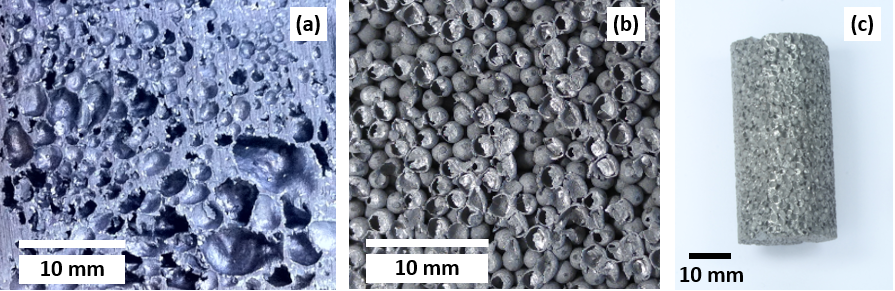
\includegraphics[width=0.95\linewidth]{Tex-Figures/Fig01a_b_c.png}
		\caption{Metallic foam samples: (a) aluminum, (b) hollow sphere steel and (c) actual steel specimen before testing. Metallic foams are cellular metals, where steel foam resembles closely packed hollow spheres.}
		\label{Samples}
	\end{center}
\end{figure}

\subsection*{Pore Size Dimensions}

The dimensions of the pores were determined to ensure that each cross-section contained a sufficient number of pores to achieve relatively homogeneous material properties. Based on a high-definition image of a transverse cut of the base samples, the largest dimension of 242 pores for HS steel foams and 237 pores for aluminum foam were measured. The 20~mm distance between the jaws of a Mitsuo digital caliper was used as a reference length for the pixel distance measurement. 726.20~pixels $=$ 20~mm in the HS steel foam, and 236.51~pixels $=$ 10~mm in the PM aluminum foam (see Figure \ref{PoreMeas}).

\begin{figure}[htbp]
	\begin{center}
		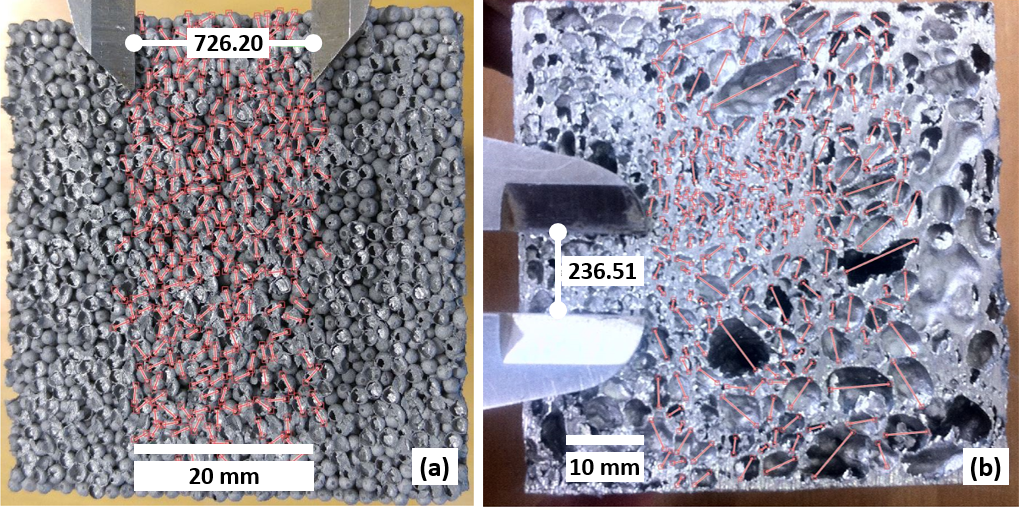
\includegraphics[width=0.80\linewidth]{Tex-Figures/Fig02a_b.png}
		\caption{Measurement of the pore size: (a) HS steel foam and (b) aluminum foam sample. Diameter of the spherical shell affects its stability and load capacity.}
		\label{PoreMeas}
	\end{center}
\end{figure}

A normal distribution with mean of 1.79~mm and variance of 0.19~mm$^2$ best described the pore sizes measured in the HS steel foam (Figure \ref{PoreSizeHistograms}a). On the other hand, the aluminum foam's pore size was best captured by a lognormal distribution with mean of 2.13~mm and variance of 1.67~mm$^2$ (Figure \ref{PoreSizeHistograms}b).

\begin{figure}
	\centering
	\begin{subfigure}{.5\textwidth}
		\centering
		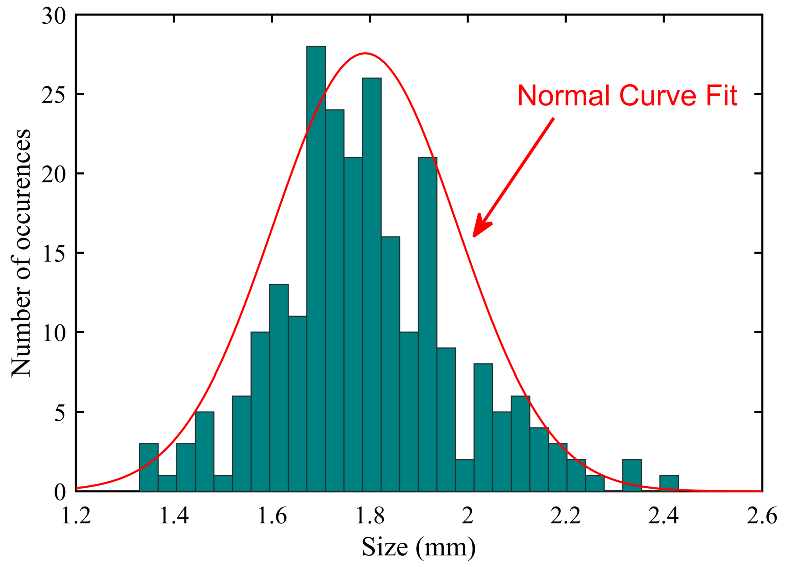
\includegraphics[width=0.95\linewidth]{Tex-Figures/Fig03a.pdf}
		\caption{Steel foam}
		\label{fig3:sub1}
	\end{subfigure}%
	\begin{subfigure}{.5\textwidth}
		\centering
		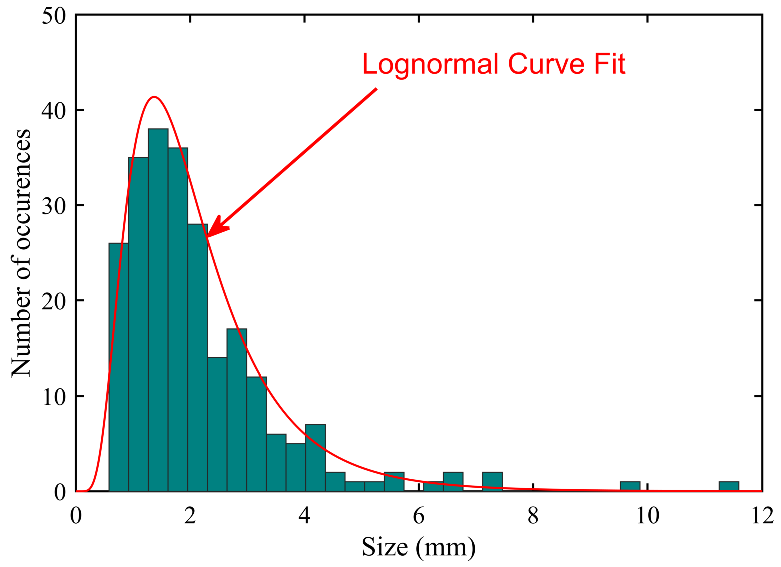
\includegraphics[width=0.95\linewidth]{Tex-Figures/Fig03b.pdf}
		\caption{Aluminum foam}
		\label{fig3:sub2}
	\end{subfigure}
	\caption{(a) Normal distribution of pore size – HS steel foam, (b) Lognormal distribution of pore size – aluminum foam. Hollow sphere foam exhibits lower variability than powder metallurgy foam, characterized by larger scatter of pore sizes.}
	\label{PoreSizeHistograms}
\end{figure}

If the pore shape is spherical, the measurement of the pore size through a transverse cut will be smaller than the pore diameter, unless the cut passes exactly through the pore's center (Figure \ref{FoamCutPlane}). Thus, an amplification factor was proposed to improve the estimate of the pore diameter from sectional pore measurements.

\begin{figure}[htbp]
	\begin{center}
		
\includegraphics[width=0.95\linewidth]{Tex-Figures/Fig04.png}
		\caption{Schematic lateral view of the cut plane on the sample. One can notice that cross-sectional diameters do not coincide with the true diameter of the sphere or cavity.}
		\label{FoamCutPlane}
	\end{center}
\end{figure}

Let us consider an unknown amplification factor as the ratio between the mean of the projected radius values and the true sphere's radius (Figure \ref{RandomPlaneCut}). If all pores are assumed as spherical, random cuts can be generated using a uniform random distribution of $h_{proj} \in \langle 0,r_{true} \rangle$ and for each cut a projected radius can be computed as:

\begin{equation}\label{Eq11}
{r_{proj}}^i=\sqrt{{r_{true}}^2-{h_{proj}^i}^2}
\end{equation}
\nomenclature{$r_{p r o j}^{i}$}{Projected Radius used for measuring the size of the spherical pore}
\nomenclature{$r_{t r u e}$}{True Radius of the spherical pore size}
\nomenclature{$h_{proj}^{i}$}{Height of the random cut plane used for measurement of the spherical pore size}

\begin{figure}[htbp]
	\begin{center}
		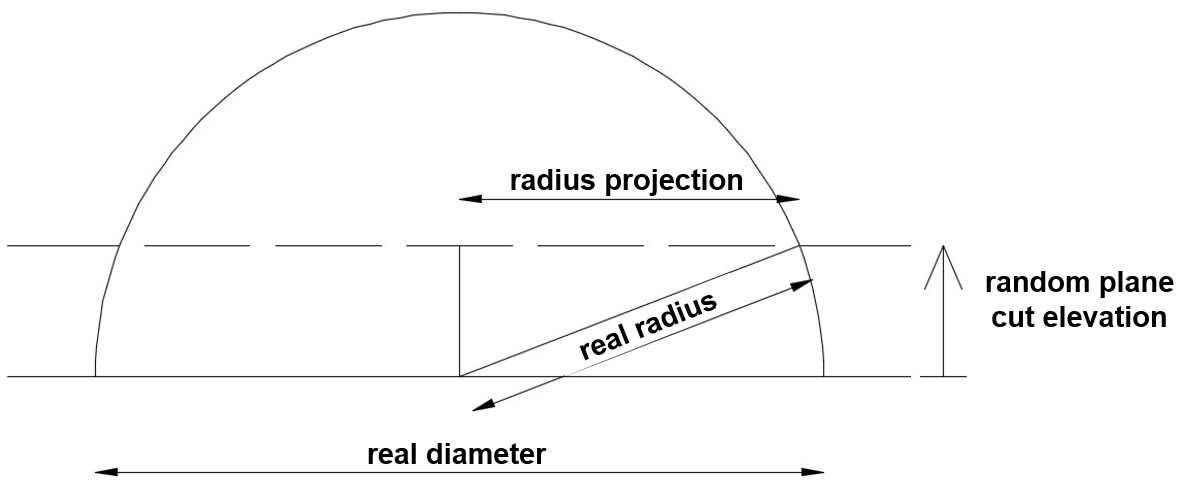
\includegraphics[width=0.75\linewidth]{Tex-Figures/Fig05.png}
		\caption{Cutting a sphere at random elevations we computed the relationship between the expected mean radius in the cut plane and the real radius of the spherical cavity.}
		\label{RandomPlaneCut}
	\end{center}
\end{figure}

Employing Monte-Carlo simulation, the average value of $\hat{r}_{proj}$ was calculated; consequently, the correction factor was calculated as:

\begin{equation}\label{Eq12}
\alpha=\frac{r_{true}}{\hat{r}_{proj}}
\end{equation}
\nomenclature{$\alpha$}{Correction factor used for the  measurement of the spherical pore size}

An amplification factor $\alpha=1.27$ was obtained. This value resulted in corrected average pore diameters of 1.27 $\times$ 1.79~mm $=$ 2.27~mm in HS steel foam and 1.27 $\times$ 2.13~mm $=$ 2.70~mm for aluminum foam, which leads us to conclude that the specimens must have at least 22~mm and 27~mm of cross-sectional width respectively. Considering the size of aluminum and steel foam blocks, specimen diameters of 25~mm were chosen as a representative for both base materials.


\section{Behavior of HS steel and PM aluminum metallic foams at elevated temperatures}

\subsection*{Mechanical testing}

Steel foam specimens were tested at 24~$^{\circ}\mathrm{C}$ (ambient temperature), 150~$^{\circ}\mathrm{C}$, 200~$^{\circ}\mathrm{C}$, 300~$^{\circ}\mathrm{C}$, 400~$^{\circ}\mathrm{C}$, 550~$^{\circ}\mathrm{C}$, and 700~$^{\circ}\mathrm{C}$, while aluminum foam specimens were tested at 24~$^{\circ}\mathrm{C}$, 150~$^{\circ}\mathrm{C}$, 200~$^{\circ}\mathrm{C}$, 300~$^{\circ}\mathrm{C}$, and 500~$^{\circ}\mathrm{C}$ (Table~\ref{Tab1}). For the most part, two specimens were tested at each temperature except ambient; one exposed to the elevated test temperature for 15~min, and the other exposed for 30~min. The exceptions were the 550~$^{\circ}\mathrm{C}$ and 700~$^{\circ}\mathrm{C}$ tests on the HS steel foam, and the 500~$^{\circ}\mathrm{C}$ test on aluminum foam, which were all exposed for only 15~min. For each test, the high-temperature furnace was heated to the test temperature without the specimen inside. Once the targeted elevated temperature was reached, the cylindrical metallic foam specimen was placed inside the furnace. The compressive test was not started until the specimen had reached and been held under a steady-state conditions at the target testing temperature for the required exposure time. The testing temperature was regulated by a thermocouple installed on the side of each specimen. \cite{Avalloneetal2007} reported that mild steel melts at a temperature of approximately 1536~$^{\circ}\mathrm{C}$, and \cite{Ashsby2000} estimated the aluminum melting temperature at approximately 660~$^{\circ}\mathrm{C}$. The majority of the testing temperatures was conducted at elevated temperatures less than 400~$^{\circ}\mathrm{C}$ because, based on both the available literature and EN 1993-1-2:2005 \cite{EC3-1-2}, the strength of steel is severely degraded at elevated temperatures exceeding 400~$^{\circ}\mathrm{C}$. The sensitivity of the mechanical properties to exposure time was evaluated by conducting the compressive testing following both 15~min and 30~min of steady-state pre-heating.

% Table generated by Excel2LaTeX from sheet 'Sheet2'
\begin{table}[htbp]
	\centering
	\caption{Temperature and exposure time during compressive experiments}
	\begin{tabular}{ccccc}
		\toprule
		{Temperature} & \multicolumn{2}{c}{Steel Foam}  & \multicolumn{2}{c}{Aluminum Foam} \\
		\midrule
		($^{\circ}\mathrm{C}$) & Melting point (\%) & Duration (min) & Melting point (\%) & Duration (min) \\
		\midrule
		24    & 2     & $\infty$     & 4     & $\infty$ \\
		150   & 10    & 15 \& 30 & 23    & 15 \& 30 \\
		200   & 13    & 15 \& 30 & 30    & 15 \& 30 \\
		300   & 20    & 15 \& 30 & 45    & 15 \& 30 \\
		400   & 27    & 15 \& 30 & -     & - \\
		500   & -     & -     & 76    & 15 \\
		550   & 37    & 15    & -     & - \\
		700   & 47    & 15    & -     & - \\
		\bottomrule
	\end{tabular}%
	\label{Tab1}%
\end{table}%

\subsection{Testing approach}

The compressive testing was conducted using a servo-hydraulic Materials Testing Systems (MTS) Model 810 Universal Testing Machine (UTM), with a capacity of 100~kN in compression. A MTS Model 652.01 High-Temperature Electric Furnace applied the thermal loads (Figure \ref{MTSFurnace}).

\begin{figure}[htbp]
	\begin{center}
		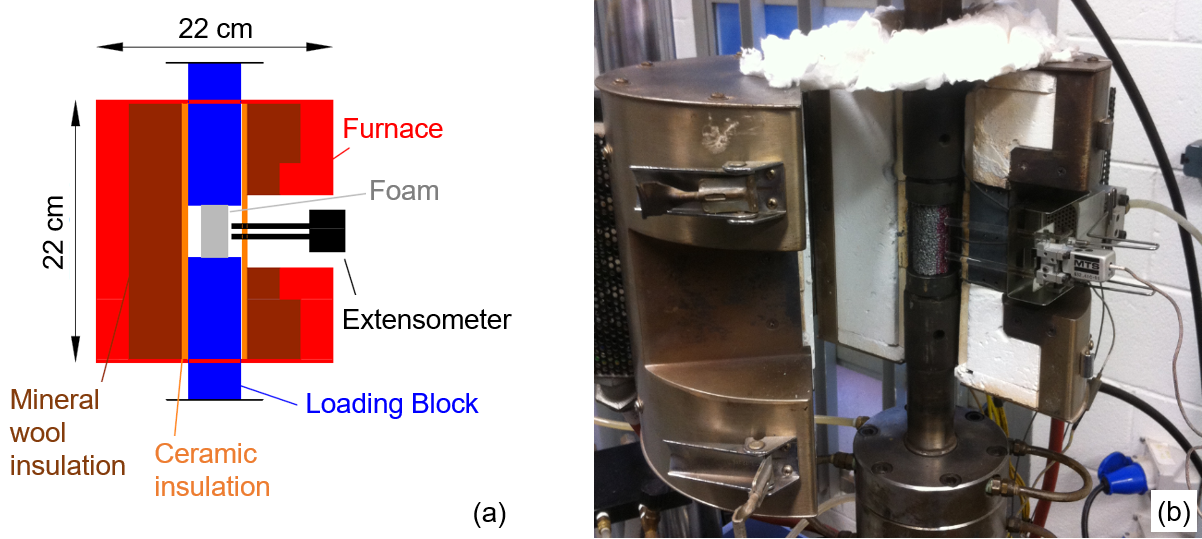
\includegraphics[width=0.95\linewidth]{Tex-Figures/Fig06.png}
		\caption{Thermal-mechanical compressive test setup: (a) annotated schematic of high-temperature furnace, and (b) Actual view of the opened furnace. Sample is heated first, and loaded after stable internal temperature is reached. Strains were measured with an extensometer inside the furnace.}
		\label{MTSFurnace}
	\end{center}
\end{figure}

Mechanical loads in the UTM were controlled using a MTS Flex Test 60 controller, and the furnace was controlled using a MTS Digital PID Temperature Controller. The high-temperature furnace allows pre-heating at temperatures up to 1000~$^{\circ}\mathrm{C}$, has multi-zone temperature control to compensate for vertical temperature gradients, and is accurate (at the constant steady-state temperature) to within $\pm$ $2\,^{\circ}\mathrm{C}$. After a preload of 0.10~kN was applied to remove any surface irregularities, axial loading was applied pseudo-statically using displacement control at a constant loading rate of 0.025~mm/s. The reported compressive stress, $\sigma$, was calculated as the ratio of the applied force $F$ to the measured cross-sectional area before loading. Ideally, the reported compressive strain $\epsilon$ would be measured using the available MTS High-Temperature Axial Extensometer. However, for many specimens the tips of the extensometer leads slipped at relatively low compressive loads, and thus for consistency the compressive strain was calculated as the ratio of crosshead displacement to the measured length of each undeformed cylindrical specimen.

\subsection{Experimental stress-strain curves}

The compressive stress-strain behavior of metallic foams exhibited three distinct phases of behavior (Figure \ref{fig:MetFoaBeh}). Until yield, the behavior was elastic (Elastic Phase), and the stress was linearly related to the strain. After yield was a large plastic plateau (Plateau Phase). Within this region, an upper and lower yield point can be identified. The final phase (Densification Phase) is characterized by densification of the metallic foam, during which the stiffness of the compressive stress-strain curve rapidly increases. During densification, the cell walls of the metallic foam begin to buckle and contact one another as the voids close. The densification phase continues until the metallic foam reaches its compressibility limit. The slope of the stress-strain curve within the densification phase is defined as the densification modulus.

\begin{figure}[htbp]
	\begin{center}
		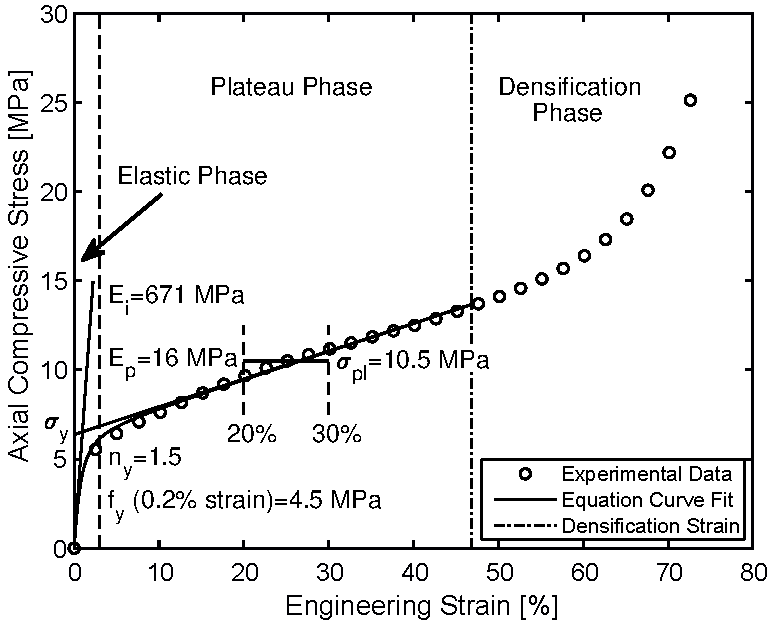
\includegraphics[width=0.75\linewidth]{Tex-Figures/Fig07.pdf}
		\caption{Parametrization of a typical, non-linear stress strain curve of metallic foam. Initial modulus corresponds to the foam stiffness, yield stress is computed at 0.2~\% strain offset, plastic hardening is the linear fit and plateau stress is the average stress within the strain range of 20~\% to 30~\%. Curvature of the transition from elastic to plastic behavior is characterized with parameter $n_y$.}
		\label{fig:MetFoaBeh}
	\end{center}
\end{figure}
\nomenclature{$E_{i}$}{Initial elastic modulus}
\nomenclature{$E_{p}$}{Plastic hardening modulus}
\nomenclature{$n_{y}$}{Shape parameter that controls the sharpness of the transition from the elastic stiffness to the plastic stiffness}
\nomenclature{$f_{y}$}{Yield stress calculated using the 0.2~\% offset strain method}
\nomenclature{$\sigma_{p l}$}{Plateau Stress}

Results from the steel and aluminum foam specimens tested under uniaxial compression at elevated temperatures are shown in Figures \ref{fig:FoamStrStr}a) and \ref{fig:FoamStrStr}b), respectively. Similar trends were observed for both types of metallic foam, in that each specimen exhibited, but to varying degrees, the three phases of behavior shown in Figure \ref{fig:MetFoaBeh}. The exposure (15~min or 30~min) did not appear to have had a systematic influence on the stress-strain behavior of the specimens. Kovacicetal \cite{Kovacicetal2016} also reported that exposure time to elevated temperature did not influence the foam's compressive behavior.

An insightful reader might notice that properties at 300~$^{\circ}\mathrm{C}$ are higher than room temperature or 100~$^{\circ}\mathrm{C}$. In addition, those from 400~$^{\circ}\mathrm{C}$ are higher than those from 200~$^{\circ}\mathrm{C}$, which might initially seem puzzling. However, a thin blue oxide film was observed to form on all cells of the steel foam specimens at temperatures exceeding 250~$^{\circ}\mathrm{C}$ (see Figure \ref{fig:BlueOxide}). The effect of steel oxidation at around 300~$^{\circ}\mathrm{C}$, the so-called ``blue brittleness effect'', is a phenomenon that occurs in steel alloys with significant Carbon content upon heating, particularly within temperatures ranging from 180~$^{\circ}\mathrm{C}$ to 370~$^{\circ}\mathrm{C}$ (\cite{XiongandLiew2016}). The blue oxide layer, which forms on the surface of the metal, is stiffer and stronger than the base steel alloy but more brittle. The addition of a stiffer film on the cells increased the macroscopic stiffness of the foam due to the large surface area relatively to the volume of the base material. The effect of the distributed stiffening of the steel foam become negligible at higher temperatures when the base steel of the cells deteriorated past the transition temperature of 400~$^{\circ}\mathrm{C}$. The effect of a blue oxide film also affected parametric properties of the stress-strain curves, such as plateau stress in the systematic analysis of the macroscopic steel foam properties at elevated temperatures described later in the paper.

\begin{figure}
	\centering
	\begin{subfigure}{.5\textwidth}
		\centering
		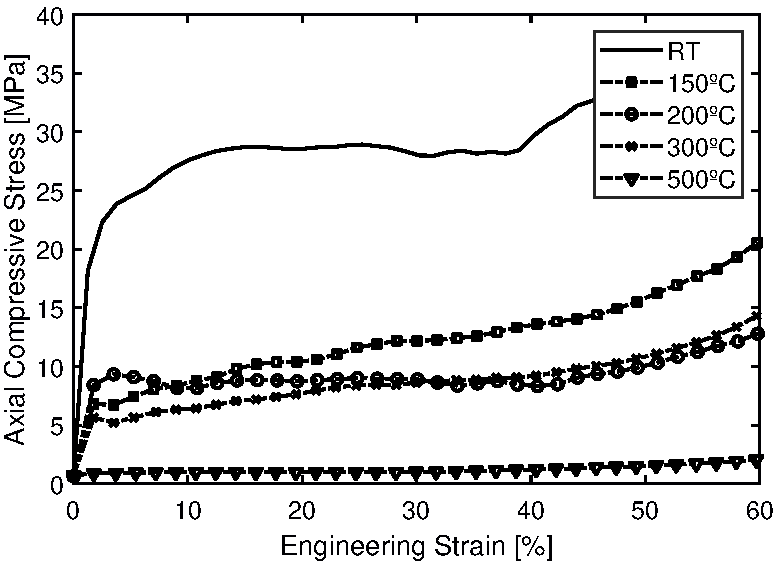
\includegraphics[width=0.98\linewidth]{Tex-Figures/Fig08a.pdf}
		\caption{Al foam}
		\label{fig8:sub1}
	\end{subfigure}%
	\begin{subfigure}{.5\textwidth}
		\centering
		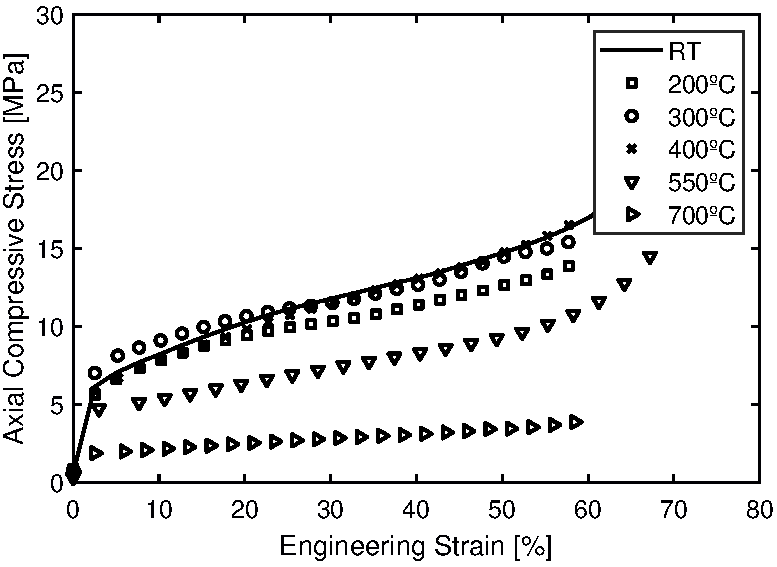
\includegraphics[width=0.98\linewidth]{Tex-Figures/Fig08b.pdf}
		\caption{Steel foam}
		\label{fig8:sub2}
	\end{subfigure}
	\caption{Stress-strain behavior of metallic foam samples as the ambient temperatures increases. Whereas Al foam loses 50\% of its capacity at 150~$^{\circ}\mathrm{C}$ only, Fe based cellular structure maintains its strength up to 400~$^{\circ}\mathrm{C}$.}
	\label{fig:FoamStrStr}
\end{figure}

\begin{figure}[htbp]
	\begin{center}
		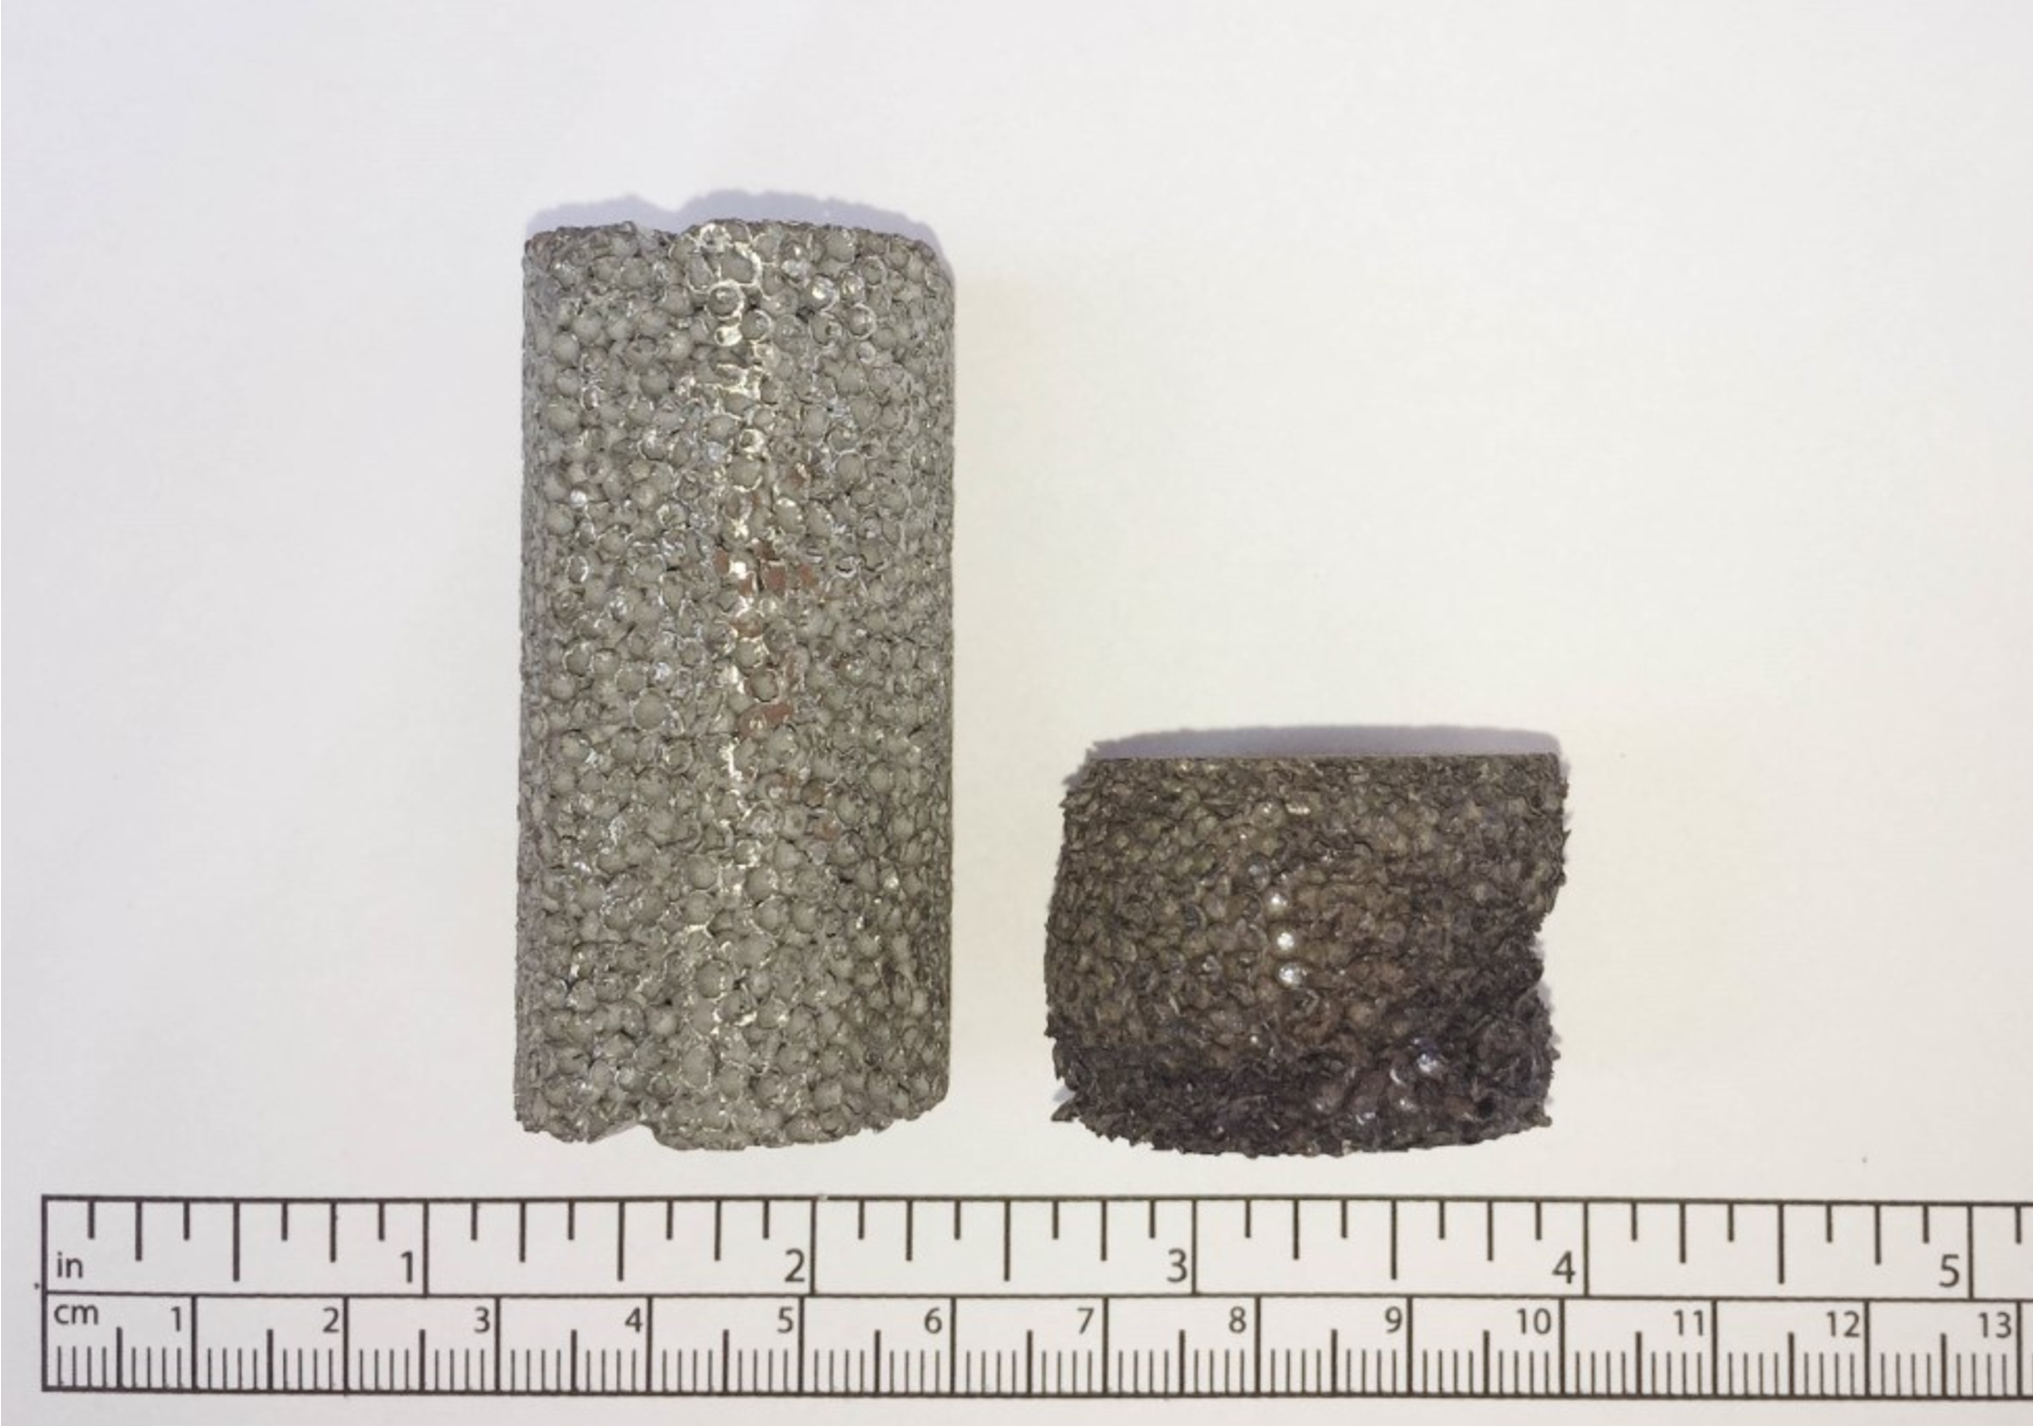
\includegraphics[width=0.75\linewidth]
		{Tex-Figures/Fig09-Blue_brittleness.pdf}
		\caption{(left) HS steel foam specimen before testing, (right) HS steel foam specimen after testing at 300~$^{\circ}\mathrm{C}$ following 30~min of exposure. Discoloration of the heated specimen indicated formation of the blue oxide film, which was highly likely stiffening the spherical shells. Formation of the stiffer oxide layer could explain better experimental performance of the steel foam samples, in comparison to the simulated predictions.}
		\label{fig:BlueOxide}
	\end{center}
\end{figure}

\FloatBarrier

\section{Micro-mechanical simulations}

The microstructure of a sintered HS foam consists of hollow spheres and welds between those spheres. The spheres have been shown to be in a random close-packed (RCP) stacking configuration \cite{Gaoetal2008}. Wouterse and Philipse \cite{WouPhi2006} tested five algorithms for generating random RCP sphere stacking and showed that two different variations of the ``Mechanical Contraction Method'' resulted in stackings that were most like an experimental stacking in their geometric properties. The algorithmically simpler of those two methods, the ``Modified Mechanical Contraction Method'', was chosen for the presented simulations, which involves the steps below. These steps are described in more detail in \cite{Kansaletal2002}, \cite{WilliamsandPhilipse2003}.

\begin{enumerate}
	\item Randomly place spheres of zero size throughout the domain.
	\item Increase the size of all spheres by an equal magnitude.
	\item Check for overlapping spheres and move both spheres in each overlap pair away from each other by an equal magnitude. Repeat this step until all but a minimum threshold of overlaps are eliminated.
	\item Repeat Steps~2 and 3 until the final sphere size is reached.
\end{enumerate}

After the spheres are successfully placed, welds are inserted to connect them. The actual welds between the spheres are solid circular shapes with concave sides which curve until they reach a tangent with the sphere. However, due to the difficulty of modeling such a shape, these welds were approximated by a straight cylinder of a given diameter connecting any spheres within a specified threshold distance. The random variables in this geometry algorithm include sphere size, wall thickness, and sphere location. The deterministic variables include the weld size, structure, and some of the input parameters for the Modified Mechanical Contraction Method such as the number of spheres to initially place and the number of overlaps threshold at which to increment the size of the spheres.

The core algorithms and functionality of the simulator was originally developed by Smith and Arwade (\cite{Smith2012,smith_characterization_2012}. The algorithm produced geometries such as that displayed in Figure \ref{Figure5}a). The original implementation used the ADINA solver, but in this study, the scripts were modified to generate meshes for LS-DYNA (\cite{hallquist_ls-dyna_2006}) due to its superior ability to handle multiple, concurrent contacts. The analyses used an implicit integration scheme for numerical efficiency and stability. The mechanical properties of the base steel at ambient temperature and 550~$^{\circ}\mathrm{C}$ as shown in Table~\ref{Tab2}. The properties are based on mechanical testing of samples with similar chemical content, namely Fe-C(0.5)-P(0.5) by Fraunhofer Institute in Dresden and independent data from World Wide Guide of Equivalent Irons and Steels (\cite{cverna_worldwide_2006}).


% Table generated by Excel2LaTeX from sheet 'Sheet2'
\begin{table}[htbp]
	\centering
	\caption{Mechanical properties employed in the simulations.}
	\begin{tabular}{ccc}
		\toprule
		\multirow{2}[0]{*}{Property} & \multicolumn{2}{c}{Value} \\
		& Ambient & $550\,^{\circ}\mathrm{C}$ \\
		\midrule
		Young modulus,~GPa & 200 & 91 \\
		Poisson ratio & 0.29  & 0.29 \\
		Yield stress,~MPa & 250 & 67.5 \\
		Ultimate strain,~mm/mm & 0.18  & 0.21 \\
		Ultimate strength,~MPa & 600 & 192 \\
		\bottomrule
	\end{tabular}%
	\label{Tab2}%
\end{table}%

The von Mises effective stress of the model under increasing compressive pressure (Figure~\ref{Figure5}b-c) indicated localized plasticity at the sphere interfaces, which led to sphere deformations. Simulated stress strain curve compared well with the experimental curve (see Figure \ref{Figure5}d).The simulated curves became irregular at large strains because the implicit algorithm used in LS-DYNA struggled to converge because of the large number of contact surfaces. The simulated curve at 550~$^{\circ}\mathrm{C}$ is noticeably higher than the experimental curve. This discrepancy is attributed to strengthening of the spherical shells due to oxidation of the steel foam at elevated temperatures (see Figure~\ref{fig:BlueOxide}). This strengthening was not accounted for in the computational model.

\begin{figure}[htbp]
	\begin{center}
		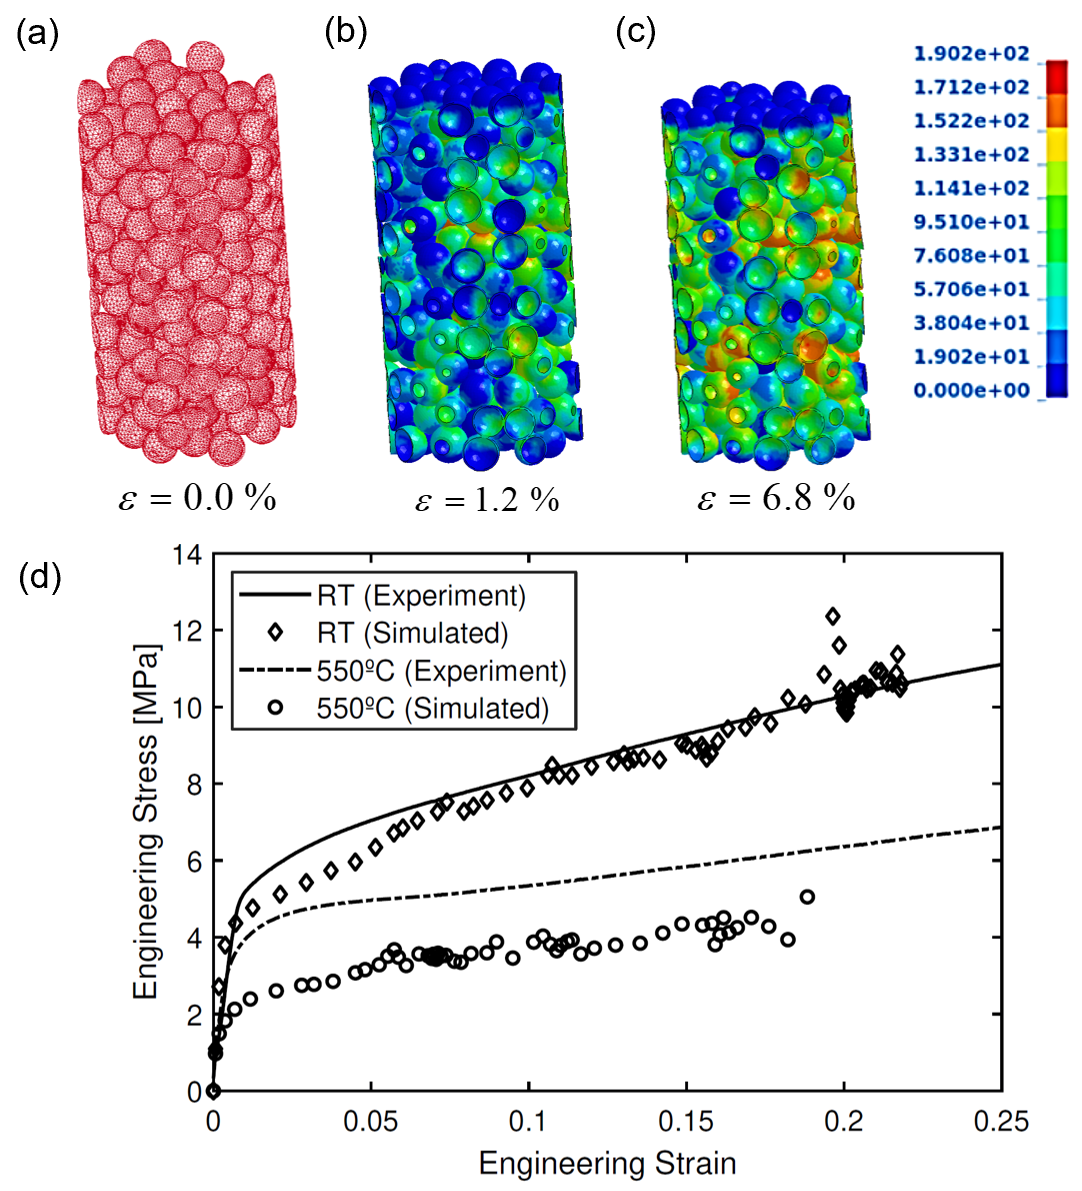
\includegraphics[width=0.75\linewidth]
		{Tex-Figures/Fig10-SimulatedCompression}
		\caption{Comparison of computational (diamonds and circles) and experimental (continuous lines) strength predictions at room (RT) and high temperature ($550\,^{\circ}\mathrm{C}$). Von Mises stress (MPa) localized in the contact regions of the hollow steel spheres. Multiple and irregular load paths followed the random packing of the spheres, which resulted from the nature of the manufacturing process. Whereas simulated and experimental data showed good agreement, steel foam samples exhibited higher stiffness and strength at high temperatures when compared to the computational prediction.}
		\label{Figure5}
	\end{center}
\end{figure}

The plastic strains localized in a few contact locations at 1.2~\% global engineering strain with progressively more localized plasticity regions with larger volume appearing at larger strains (Figure \ref{Fig:SimulatedBuckling}a-c). The randomness and tortuosity of the internal load paths is consistent with experimental study by Gr\"{u}nder et al. \cite{grunder_modeling_2001}. They tracked increasing contact areas between the spheres using CT images, while increasing the compressive loads. The location of the contact areas and direction of the local load paths changed from sphere to sphere in a random, chaotic manner. It is consistent with our simulated cross-sections in the micro-model. Figure \ref{Fig:SimulatedBuckling}d-f illustrate the typical deformation mechanism of the individual spheres. Even though only cross-sections are shown, these deformations are 3-dimensional and mostly axi-symmetric. The key parameters identified by \cite{Fallet2008}, such as sphere radius $R$, thickness $t$, diameter of the contact area, and degraded mechanical properties of the base metal are all significant. The simulations showed that the diameter of the contact area was not constant; it gradually increased until the sphere collapsed at large strains. The simulations clearly indicated that plasticity dominated the local deformations of our HS steel foam samples.

\begin{figure}[htbp]
	\begin{center}
		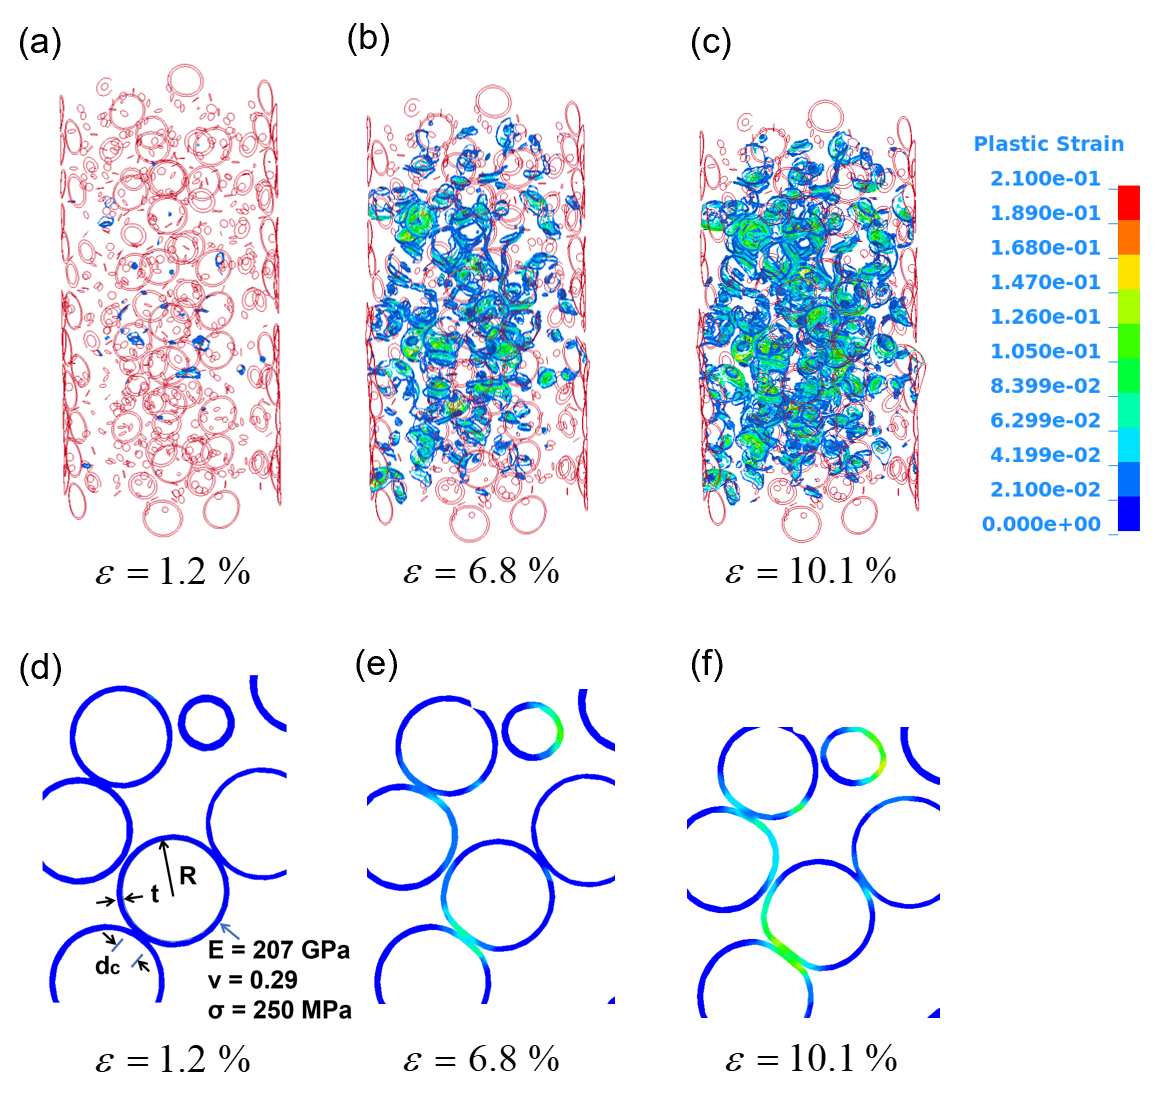
\includegraphics[width=0.80\linewidth]
		{Tex-Figures/Fig11-PlasticBuckling.png}
		\caption{Plasticity localized at sphere interfaces experiencing plastic deformations arising from contact forces. As the load increased, the number of contact pairs and subsequently, plastic regions surged (b-c). Radius, $R$ and thickness, $t$ of the spherical shell, the diameter of the contact interface, $d_c$ and material properties of the hollow spheres influence the local resistance mechanism (d). Following the initial yielding around the contact region, the plasticity spreads toward the equator of the sphere, accompanied by the gradually increasing diameter of the plastic hinge hoop moving outwards from the initial contact area (e-f). Due to the random packing, the number of contact regions and their directions vary from sphere to sphere, which is consistent with experimental study reported by Fallet et al. \cite{Fallet2008}.}
		\label{Fig:SimulatedBuckling}
	\end{center}
\end{figure}


\subsection{Insights from the analytical expressions for buckling of a spherical shell}

Pressure applied to a sphere, $q_c$ needs to satisfy equilibrium with the membrane stress within the walls of the spherical shell \cite{TimGer2009}:

\begin{equation}\label{Eq1}
\sigma_{shell}2\pi Rt=q_c\pi \frac{{d_c}^{2}}{4}
\end{equation}
\nomenclature{$R$}{Sphere radius}
\nomenclature{$t$}{Sphere Thickness}
\nomenclature{$\sigma_{shell}$}{Buckling Stress of Spherical Shell}
\nomenclature{$q_{c}$}{Pressure applied to a sphere}
\nomenclature{$d_{c}$}{Diameter of the contact area between the spheres}

Thus, the membrane stress resulting from the applied pressure can be approximated as:

\begin{equation}\label{Eq2}
\sigma_{shell}=q_c\frac{{d_c}^{2}}{8Rt}
\end{equation}

When the critical limit of the membrane stress is exceeded, it may fail either due to material yielding at the elastic limit, $\sigma_y$, or due to the buckling arising from its geometric imperfections. The shell's stress limit to avoid the elastic buckling is taken from \cite{TimGer2009} as:

\begin{equation}\label{Eq3}
\sigma_{cr}=\frac{Et}{R\sqrt{3(1-\nu^2)}}
\end{equation}
\nomenclature{$\sigma_{c r}$}{Critical limit of membrane stress}
\nomenclature{$E$}{Young Modulus}
\nomenclature{$\mathcal{V}$}{Poisson ratio}

Yielding typically leads to geometrical buckling anyway and the loss of the ideal spherical shape. Thus, the shell capacity of a hollow sphere can be expressed as:

\begin{equation}\label{Eq4}
\sigma_\text{failure}=\min(\sigma_y,\sigma_{cr})
\end{equation}
\nomenclature{$\sigma_\text{failure}$}{Failure stress}
\nomenclature{$\sigma_{y}$}{Yield stress}

In the simulations, the steel base metal had a modulus of elasticity of $E=200$~GPa, Poisson's ratio of $v=0.29$, and yield stress of $\sigma_y=250$~MPa. The average radius and thickness of the spheres were reported in a previous study \cite{Szyniszewskietal2014} as $R = 1.86$~mm and $t = 0.02$~mm, respectively. The resulting geometrical slenderness, expressed as the ratio of the radius to the thickness, $R/t = 93$, is consistent with the plastic buckling region (Figure \ref{fig12:sub1}). A more general measure of the slenderness is the ratio of the plastic yield stress to the elastic buckling stress because it includes the influence of the material properties on the slenderness:

\begin{equation}\label{Eq5}
\lambda=\frac{\sigma_y}{\sigma_{cr}}
\end{equation}
\nomenclature{$\lambda$}{Slenderness}

If slenderness $\lambda<1$, then the structure is controlled by the material failure, namely plastic yielding. Alternatively, $\lambda>1$ indicates high slenderness and propensity for elastic buckling (Figure~\ref{fig12:sub2}). Winter \cite{Winter1947} developed an empirical curve for metallic plates, which showed that the transition between plastic and elastic buckling capacities is more gradual, and that there exists additional post-buckling reserve capacity in the elastic buckling regime. Even considering Winter's curve, the HS steel foam, as well as other foams reported by \cite{Fallet2008}, are still controlled by plastic buckling.

Coincidentally, the elastic buckling equations of a spherical shell also describes the elastic buckling capacity of a circular shell. Thus, the buckling curve in Figure~\ref{fig12:sub2} can also be used to analyzed hollow tubular lattice structures. Even considering the lightest metallic material achieved to-date by Schaedler et al. \cite{Sch2011}, only one of their configurations was in the elastic buckling region. Schaedler's experiments showed that the slender lattice exhibited large, reversible deformations, while the stub lattices experienced non-reversible deformations but higher absolute strength. These experimental observations are consistent with plastic and elastic buckling of the cylindrical shells at the junctions of the hollow tubular struts.

\begin{figure}[htp]
	\centering
	\begin{subfigure}{0.95\textwidth}
		\centering
		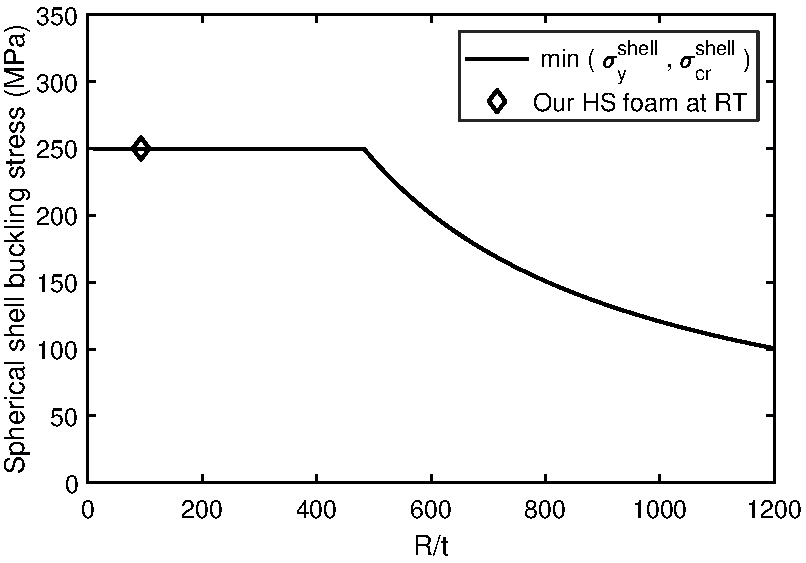
\includegraphics[width=0.65\linewidth]
		{Tex-Figures/Fig12a_Buckling_b_t.pdf}
		\caption{The effect of geometric slenderness on the buckling capacity of a single sphere.}
		\label{fig12:sub1}
	\end{subfigure}

	\par\bigskip % force a bit of vertical whitespace

	\begin{subfigure}{0.95\textwidth}
		\centering
		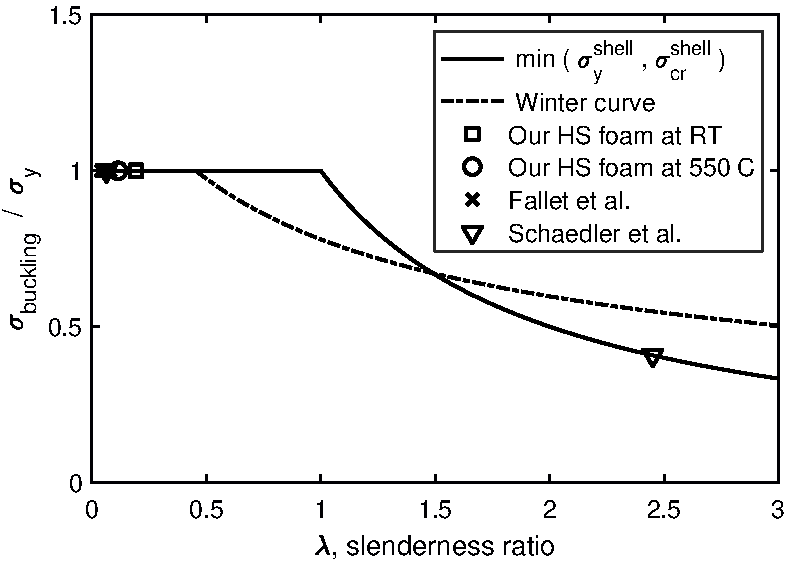
\includegraphics[width=0.65\linewidth]
		{Tex-Figures/Fig12b_Buckling_lambda.pdf}
		\caption{The effect of slenderness ratio on the buckling strength of a hollow sphere.}
		\label{fig12:sub2}
	\end{subfigure}
	\caption{Buckling capacity of a single spherical shell expressed in terms of its critical membrane stress. Geometric slenderness of our hollow sphere steel foam expressed as the ratio of radius to thickness, R/t is low and consistent with the plastic buckling mechanism. Normalized theoretical buckling stress as a function of the non-dimensional slenderness parameter, $\lambda$ overlaid with a range of theoretical capacities of foams and tubular lattice structures. Apart from the ultra-light metallic lattice, most of the manufactured cellular structures have very low slenderness, which is consistent with the irreversible, plastic buckling.}
\end{figure}

\nomenclature{$\sigma_{y}^{shell}$}{Yield stress of the spherical shell}
\nomenclature{$\sigma_{cr}^{shell}$}{Critical stress of the spherical shell}

Based on a review of available data, conventionally produced HS foams exhibit local deformation mechanism controlled by the plastic buckling of the spherical shells. Thus, the thermal degradation of the global mechanical properties of our HS foam specimens is anticipated to be controlled by the influence of elevated temperatures on the base metal's yield stress.

\FloatBarrier

Regarding the influence of the temperature on the stiffness of the foam, radial displacement of a spherical shell under uniform external pressure, $q$ is a function of its geometry and elastic constants \cite{TimGer2009}:

\begin{equation}\label{Eq6}
w(\varphi)=\frac{q(1+\nu)R^2}{Et}\left [ k(\varphi)\cot\varphi+\cos \varphi- \frac{1}{1+\cos\varphi} \right ]
\end{equation}
\nomenclature{q}{Applied pressure}
\nomenclature{$\varphi$}{Polar coordinate, where 0 corresponds to the equator and \pi/2 to the apex of the sphere}

where $k(\varphi)$ is the auxiliary variable:

\begin{equation}\label{Eq7}
k(\varphi)=\left ( 1- \frac{1}{1+\cos\varphi} + \log(1+\cos\varphi) \right ) \sin \varphi
\end{equation}

The deformation of the apex corresponds to $\varphi=\frac{\pi}{2}$, which gives:

\begin{equation}\label{Eq8}
w_{apex}=-\frac{q(1+\nu)R^2}{Et}
\end{equation}
\nomenclature{$\omega_{a p e x}$}{Deformation of the sphere apex under uniform pressure}

Since the direct influences of temperature on the radius and thickness of the sphere, as well as Poisson's ratio, are expected to be minimal, the thermal degradation of the foam stiffness is anticipated to be controlled by the base metal's modulus of elasticity.

\section{Standard Metrics Calculated based on ISO Standard 13314:2011}

The following sections synthesize experimental observations to reveal the trends of the macroscopic material properties such as the plateau stress and ambient-temperature modulus of elasticity. Based on the computational and analytical considerations described in Section~3, it was anticipated that the phenomenological properties of the HS foam, with stub spherical shells, would primarily reflect the thermal degradation trends of their base metals' plastic properties.

\subsection{Yield Strength}

Porous metallic materials are known to exhibit substantial plastic yielding capacity following an initial elastic phase, but they do not typically exhibit a ``yield plateau''. Therefore, ISO Standard 13314:2011 recommends using the 0.2~\% strain offset method to calculate the quasi-elastic compressive yield strength of porous metallic materials. Figure \ref{Quasi-elastic_modulus} show the retained yield strength of the HS steel and PM aluminum foams. At temperatures at or below 400~$^{\circ}\mathrm{C}$ the HS steel foam retained an average of about 80~\% of its ambient-temperature yield strength, but at temperatures exceeding 400~$^{\circ}\mathrm{C}$ the yield strength was significantly degraded. The PM aluminum foam retained an average of less than 50~\% of its ambient-temperature yield strength at or below 200~$^{\circ}\mathrm{C}$, and the retained yield strength was only 4.4~\% at 500~$^{\circ}\mathrm{C}$.

\begin{figure}
	\centering
	\begin{subfigure}{.5\textwidth}
		\centering
		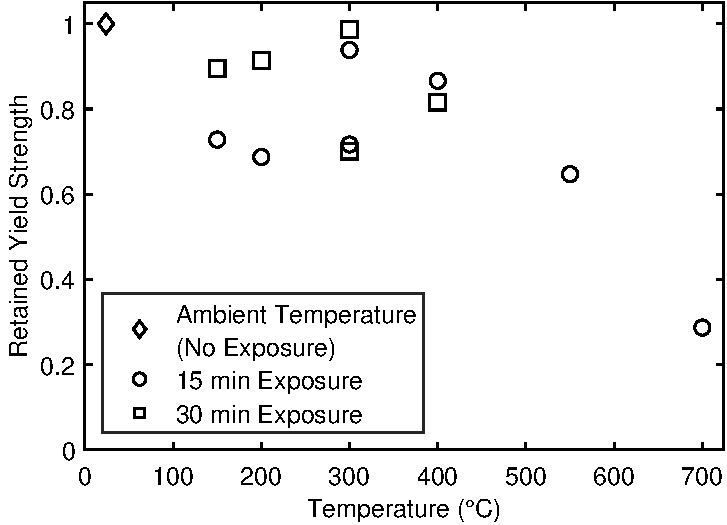
\includegraphics[width=0.95\linewidth]
		{Tex-Figures/Fig13a-yield_stress.pdf}
		\caption{Steel foam}
		\label{fig3:sub1}
	\end{subfigure}%
	\begin{subfigure}{.5\textwidth}
		\centering
		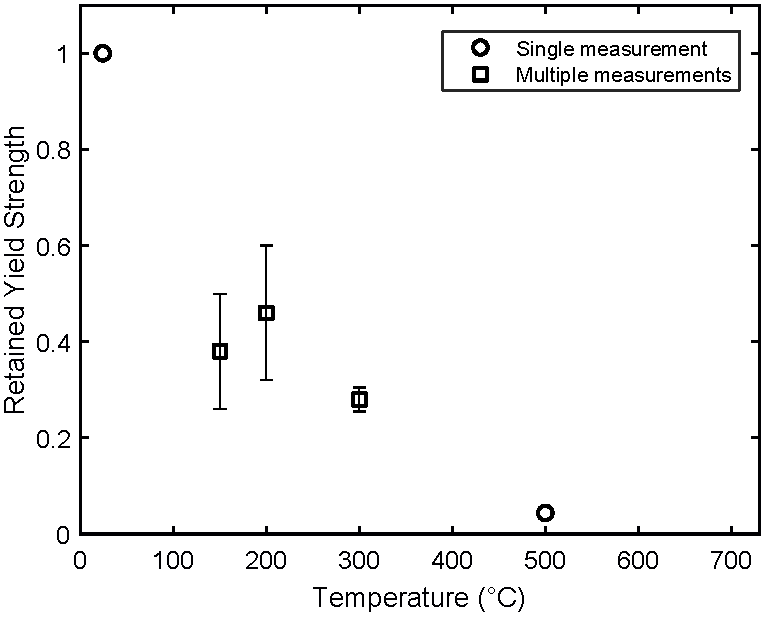
\includegraphics[width=0.95\linewidth]
		{Tex-Figures/Fig13b-yield_stress.pdf}
		\caption{Aluminum foam}
		\label{fig3:sub2}
	\end{subfigure}
	\caption{Retained quasi-elastic modulus (i.e., the ratio of the quasi-elastic modulus for a specimen tested at temperature $T>T_\text{amb}$ to that of a specimen tested at ambient temperature). The quasi-elastic modulus is the the initial slope of the elastic phase of the compressive stress-strain curve. Elastic modulus degrades noticeably at 700~$^{\circ}\mathrm{C}$ for steel foam, and at 150~$^{\circ}\mathrm{C}$ for Aluminum foam}
	\label{Quasi-elastic_modulus}
\end{figure}


\subsection{Plateau Stress}

The plateau stress, shown in Figure \ref{Plateu_stress}, was calculated following ISO Standard 13314:2011 as the average value of the stresses within the strain range spanning from 0.20~mm/mm and 0.30~mm/mm. There was little degradation in the measured plateau stress of the HS steel foam specimens at or below a 400~$^{\circ}\mathrm{C}$. However, the plateau stress of the PM aluminum foam specimens had significantly degraded by approximately 50~\% at only 150~$^{\circ}\mathrm{C}$ (i.e., at only 23~\% of aluminum's melting point).


\begin{figure}
	\centering
	\begin{subfigure}{.5\textwidth}
		\centering
		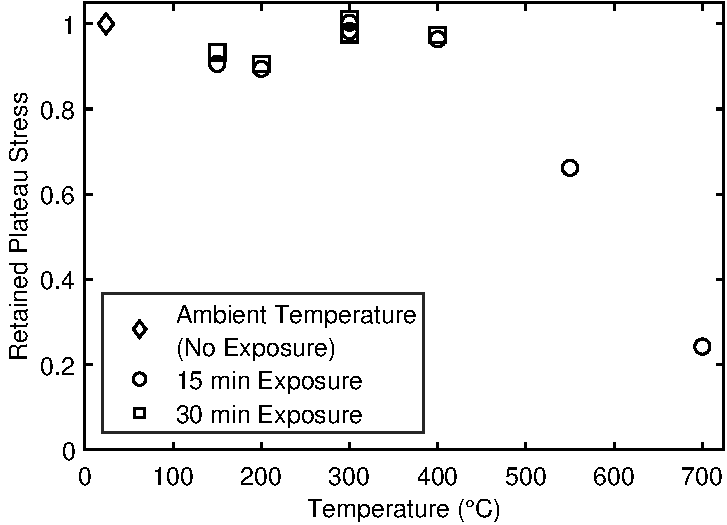
\includegraphics[width=0.95\linewidth]
		{Tex-Figures/Fig14a-plateau_stress.pdf}
		\caption{Steel foam}
		\label{fig3:sub1}
	\end{subfigure}%
	\begin{subfigure}{.5\textwidth}
		\centering
		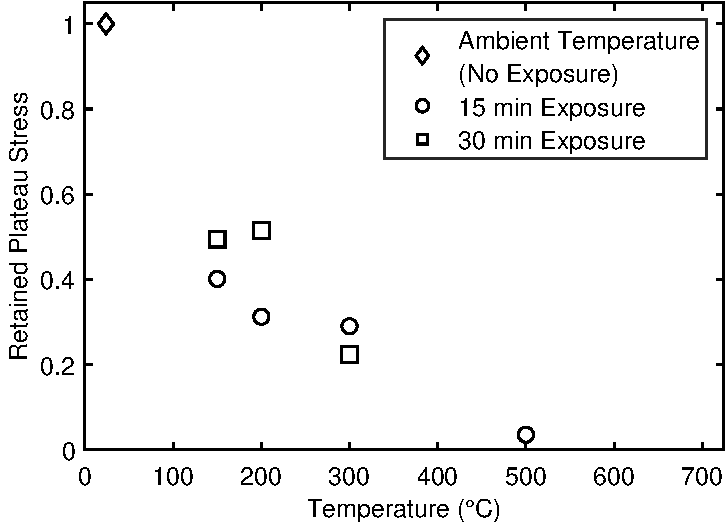
\includegraphics[width=0.95\linewidth]
		{Tex-Figures/Fig14b-plateau_stress.pdf}
		\caption{Aluminum foam}
		\label{fig3:sub2}
	\end{subfigure}
	\caption{Retained plateau stress (i.e., the average stress in the range of 20~\% to 30~\% engineering strain) of a specimen tested at temperature $T>T_\text{amb}$ to that of a specimen tested at ambient temperature. The plateau stress degrades noticeably at 550~$^{\circ}\mathrm{C}$ for steel foam, and at 150~$^{\circ}\mathrm{C}$ for Al foam.}
	\label{Plateu_stress}
\end{figure}

The exposure (15~min or 30~min) had relatively little influence on the retained plateau stress for the HS steel foam; the retained plateau stress for the two exposures did not differ by more than 4.0~\%. The retained plateau stress of the PM aluminum foam was more scattered, but no systematic influence of exposure on the energy absorption capacity was observed. It was noted that the porosity of the PM aluminum foam specimens ranged from 71.4~\% to 81.8~\%, which may have increased the variability in their calculated mechanical properties, relative to those for the HS steel foam specimens.

\subsection{Additional Metrics Calculated based on Multi-Parameter Curve Fit}

To further characterize the response of the HS steel and aluminum foams, the nine-parameter phenomenological equation

\begin{equation}\label{Eq9}
\sigma(\varepsilon,T)=\left\{\begin{matrix}
\frac{\big(E_i(T)-E_p(T)\varepsilon\big)}{{\Bigg(1+\left | \frac{\big(E_i(T)-E_p(T)\varepsilon\big)}{\sigma_y(T)} \right |^{n_y(T)}\Bigg)}^{\Big(\frac{1}{n_y(T)}\Big)}} + E_p(T)\varepsilon, & \varepsilon\leq \varepsilon_d\\
\sigma_d+ \frac{\big(E_b(T)-E_d(T)\big)\big(\varepsilon-\varepsilon_d(T)\big)}{{\Bigg(1+\left | \frac{\big(E_b(T)-E_d(T)\big)\big(\varepsilon-\varepsilon_d(T)\big)}{\sigma_p(T)} \right |^{n_b(T)}\Bigg)}^{\Big(\frac{1}{n_b(T)}\Big)}} + E_d(T)\big(\varepsilon-\varepsilon_d(T)\big), & \varepsilon> \varepsilon_d
\end{matrix}\right.
\end{equation}
\nomenclature{$\sigma_{d}$}{Densification Stress that define the transition to stiffening behavior}
\nomenclature{$E_{i}(\mathrm{T})$}{Initial elastic modulus at high temperature}
\nomenclature{$E_{p}(\mathrm{T})$}{Plastic hardening modulus at high temperature}
\nomenclature{$\varepsilon$}{Compressive strain}
\nomenclature{$\varepsilon_{d}$}{Densification Strain that define the transition to stiffening behavior}
\nomenclature{$E_{b}(\mathrm{T})$}{Slope of the segment, which constraints Richard's equation fir at the densification point $(\epsilon_d,\sigma_d)$ , which is obtained by minimizing the square area between the fitted curve and the experimental data}
\nomenclature{$E_{d}(\mathrm{T})$}{Densification stiffness}
\nomenclature{$\varepsilon_{d}(\mathrm{T})$}{Densification stiffness}
\nomenclature{$\sigma_{p}(\mathrm{T})$}{Projection of densification stress at zero strain}
\nomenclature{$n_{b}(T)$}{Shape parameter that controls the sharpness of the transition from the plastic stiffness  to the densification stiffness  at high temperature, Figure 7}
\nomenclature{$n_{y}(T)$}{Shape parameter that controls the sharpness of the transition from the elastic stiffness  to the plastic stiffness  at high temperature}
\nomenclature{$T$}{Temperature}

where
\begin{equation}\label{Eq10}
\sigma_d(T)= \frac{\big(E_i(T)-E_p(T)\big)\varepsilon_d(T)}{{\Bigg(1+\left | \frac{\big(E_i(T)-E_p(T)\big)\varepsilon_d(T)}{\sigma_p(T)} \right |^{n_y(T)}\Bigg)}^{\Big(\frac{1}{n_y(T)}\Big)}} + E_p(T)\varepsilon_d(T),
\end{equation}

was fitted to the compressive stress-strain response of each specimen. Similar five-parameter models have been successfully used in previous research to characterize the thermal-structural performance of structural components, such as high-strength bolts (see \cite{Wei2018}). Equation~\ref{Eq9} is piecewise; each of the two segments is based on the nonlinear four-parameter ``Richard Equation'', which was formulated in \cite{Ric1975}. In Equations~\ref{Eq9} and \ref{Eq10}, $\sigma$ is the compressive stress, $\varepsilon$ is the compressive strain, $E_i$ and $E_p$ are initial elastic and plastic hardening modulus of the stress-strain response, respectively; $E_b$ It is a slope of the segment, which constraints Richard's equation fir at the densification point $(\varepsilon_d,~\sigma_d)$, which is obtained by minimizing the square area between the fitted curve and the experimental data. $\sigma_y$ is a reference load that corresponds to the projection of the plastic modulus at zero strain, $n_y$ is a shape parameter that controls the sharpness of the transition from the elastic stiffness to the plastic stiffness, $\varepsilon_d$ is the densification strain, ($\varepsilon_d$, $\sigma_d$) are the stress-stain coordinates of the inflection point defining the transition to stiffening behavior, $\sigma_p$ is the projection of the densification stress at zero strain, $n_d$ is a shape parameter controlling the sharpness of the transition from the plastic stiffness to the densification stiffness $E_d$, and $(T)$ denotes dependence of the stiffness or capacity parameter on temperature.

The fitted values for the parameters in Equation~\ref{Eq9} were determined using constrained gradient-based nonlinear multivariable optimization techniques available in MATLAB's Optimization Toolbox (\cite{Mat}). Tables~\ref{Tab3} and \ref{Tab4} (located in the appendix) presents a summary of the final fitted parameters for each individual foam specimen, and quality of the analytical fits is also shown in Figure~\ref{fig:Stress_strain_fit}. Discussion on each of the calculated parameters is provided in the following sections.

\begin{figure}
	\centering
	\begin{subfigure}{1.00\textwidth}
		\centering
		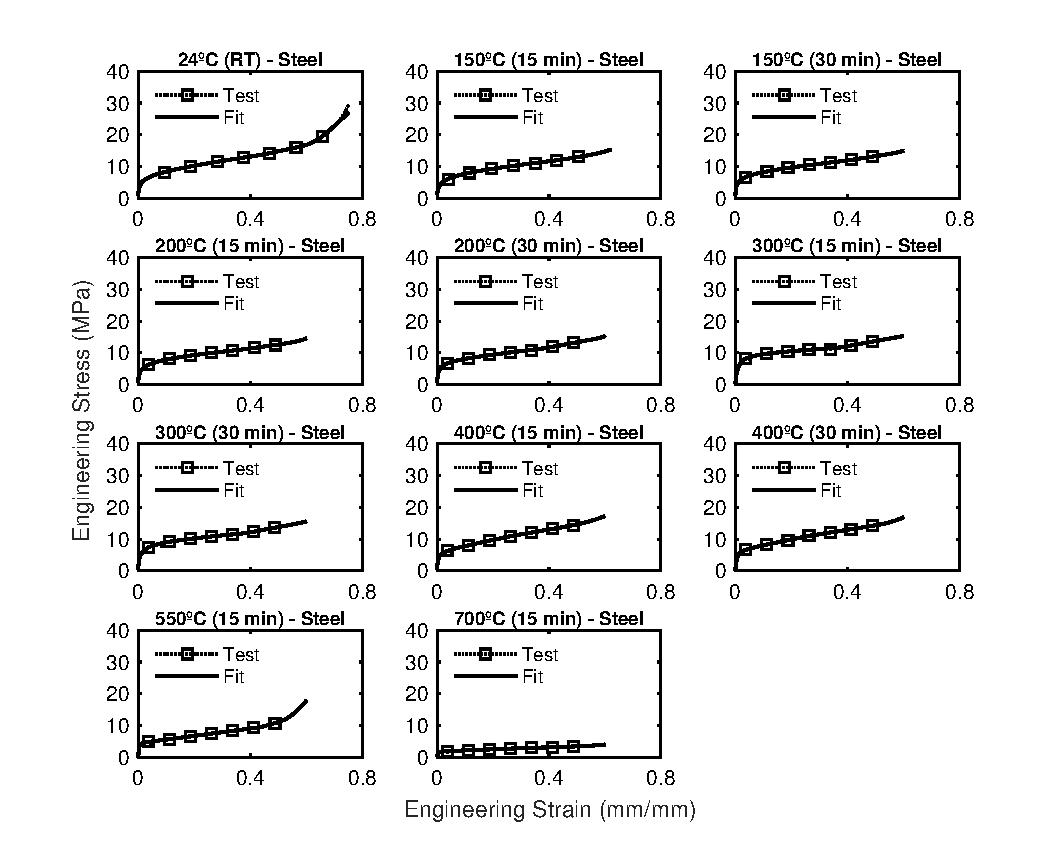
\includegraphics[width=0.90\linewidth]
		{Tex-Figures/Fig15a-StressStrain-fit-Fe.pdf}
		\caption{Steel foam}
		\label{fig:StressStrain_Rich_Steel}
	\end{subfigure}

	\par\bigskip % force a bit of vertical whitespace

	\begin{subfigure}{1.00\textwidth}
		\centering
		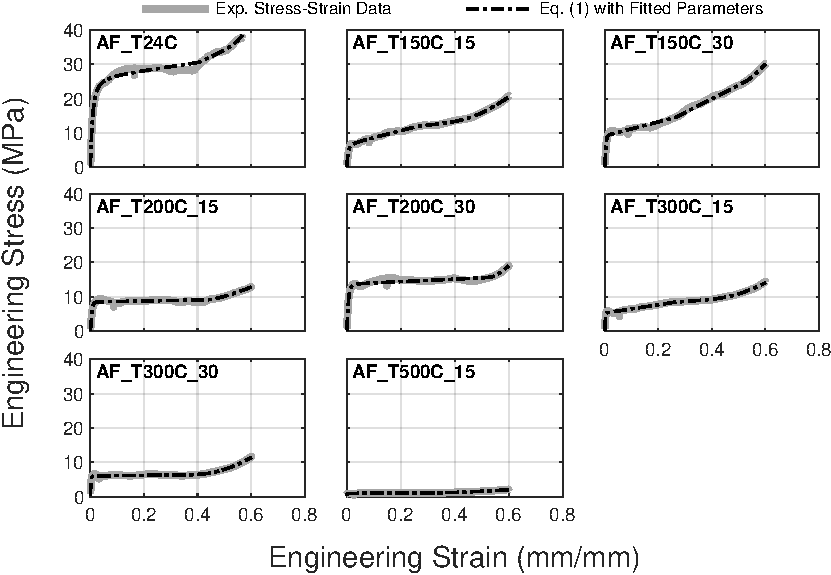
\includegraphics[width=0.70\linewidth]
		{Tex-Figures/Fig15b-StressStrain-fit-Al.pdf}
		\caption{Aluminum foam}
		\label{fig:StressStrain_Rich_Al}
	\end{subfigure}
	\caption{Equation~(9) fitted to the full stress-strain behavior of each specimen for: (a) HS steel foam specimens, and (b) PM aluminum foam specimens. Each plot is denoted by specimen name, using an annotation located in the upper-left-hand corner.}
	\label{fig:Stress_strain_fit}
\end{figure}


\subsubsection{Quasi-Elastic Modulus}

The quasi-elastic modulus is the initial slope of the elastic phase of the compressive stress-strain curve. It should be noted that the definition of the quasi-elastic modulus differs slightly from that of the elastic gradient, which can be calculated only after the specimen has been loaded and subsequently unloaded. The quasi-elastic modulus was calculated by fitting Equation~\ref{Eq9} within $[0, \varepsilon_y]$, where $\varepsilon_y$ is the yield strain calculated using the 0.2~\% offset method recommended by ISO Standard 13314:2011. Figures \ref{fig:qElas_Rich_Steel} and \ref{fig:qElas_Rich_Al} show Equation~\ref{Eq9}, with fitted parameters calculated using structural optimization techniques, relative to the stress-strain data in the elastic phase. Obviously, Equation~\ref{Eq9} can provide a very close approximation to the actual experimental data. The fitted parameter values for each specimen are provided in the appendix.
\nomenclature{$\varepsilon_{y}$}{Yield strain calculated using the 0.2~\% offset method}


\begin{figure}
	\centering
	\begin{subfigure}{1.00\textwidth}
		\centering
		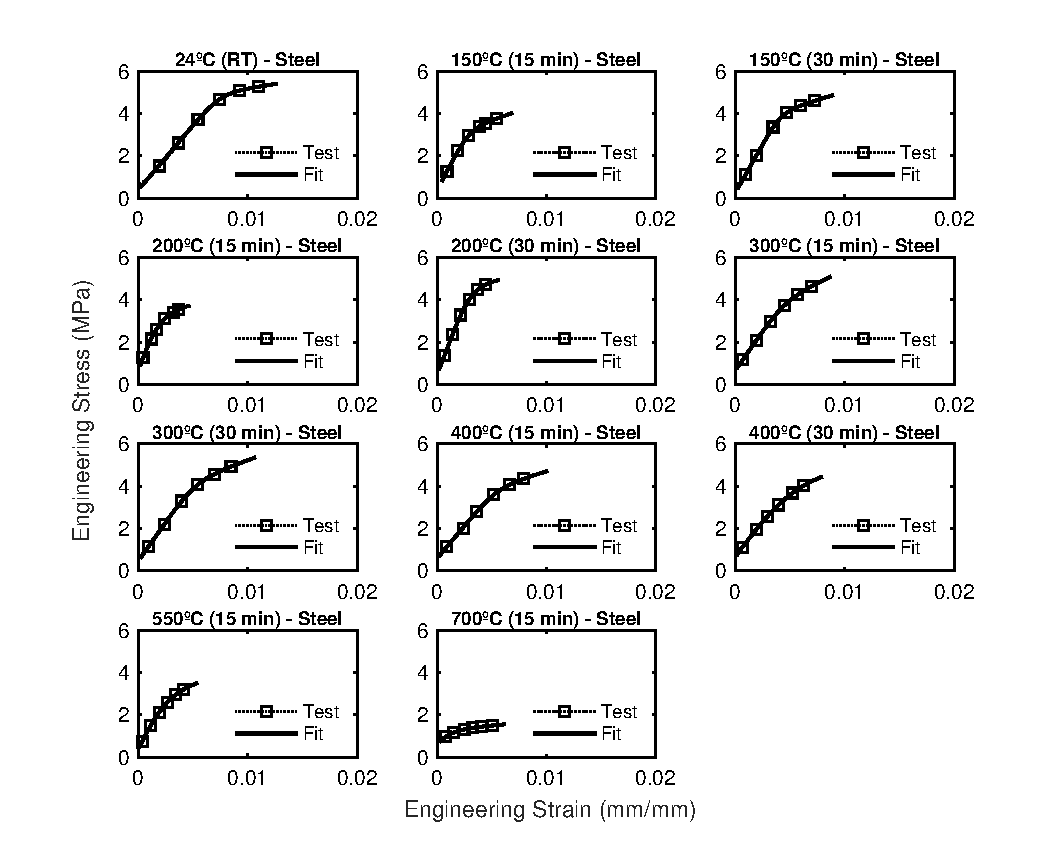
\includegraphics[width=0.90\linewidth]
		{Tex-Figures/Fig16a-quasi-Elastic-fit-Fe.pdf}
		\caption{Steel foam}
		\label{fig:qElas_Rich_Steel}
	\end{subfigure}

	\par\bigskip % force a bit of vertical whitespace

	\begin{subfigure}{1.00\textwidth}
		\centering
		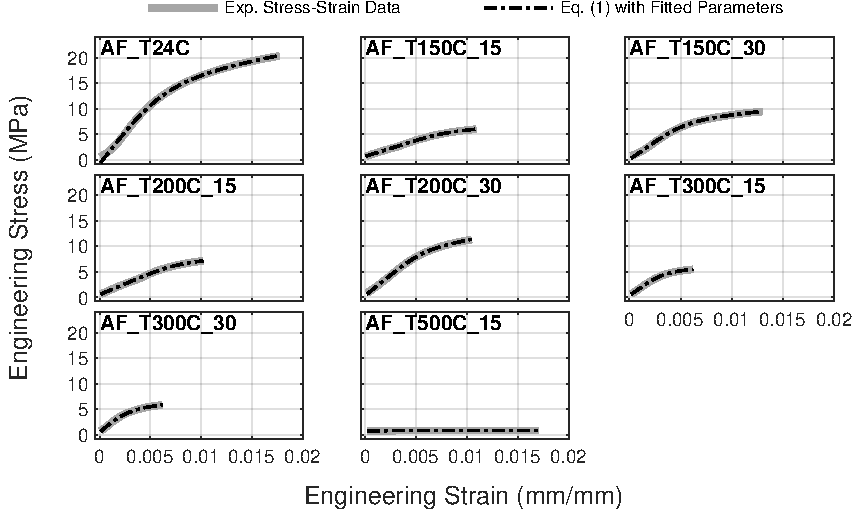
\includegraphics[width=0.70\linewidth]
		{Tex-Figures/Fig16b-quasi-Elastic-fit-Al.pdf}
		\caption{Aluminum foam}
		\label{fig:qElas_Rich_Al}
	\end{subfigure}
	\caption{ Equation~(9) fitted to the the initial strain range of the stress strain curve for: (a) HS steel foam specimens, and (b) PM aluminum foam specimens. Each plot is denoted by specimen name, using an annotation located in the upper-left-hand corner.}
	\label{fig:Stress_strain_elast_fit}
\end{figure}

Figure \ref{fig:Quasi-elast-modulus} show the resulting retained quasi-elastic modulus as a function of temperature. While values for the retained quasi-elastic modulus of the HS steel foam were widely scattered, the quasi-elastic modulus did not degrade noticeably with increasing temperature (i.e., the value of the retained quasi-elastic modulus was greater than 1.0 across the entire temperature range). The largest increases in retained quasi-elastic modulus were at $200^{\circ}\mathrm{C}$ and $300^{\circ}\mathrm{C}$. Conversely, quasi-elastic modulus of Aluminum foam deteriorated rapidly with the increase of the ambient temperature.


\begin{figure}
	\centering
	\begin{subfigure}{0.50\textwidth}
		\centering
		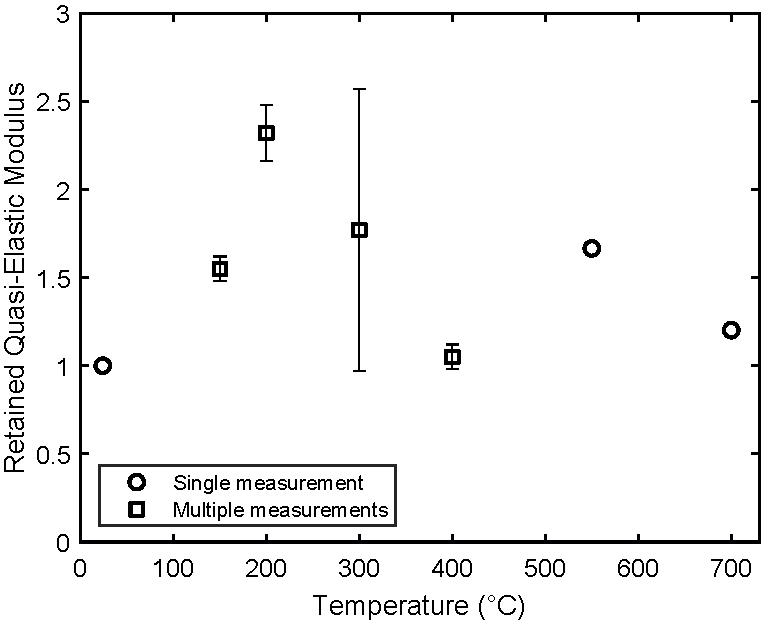
\includegraphics[width=0.90\linewidth]
		{Tex-Figures/Fig17a-qElast-Fe.pdf}
		\caption{Steel foam}
		\label{fig:Quasi-elast-modulus_Steel}
	\end{subfigure}% need comment here
	\begin{subfigure}{0.50\textwidth}
		\centering
		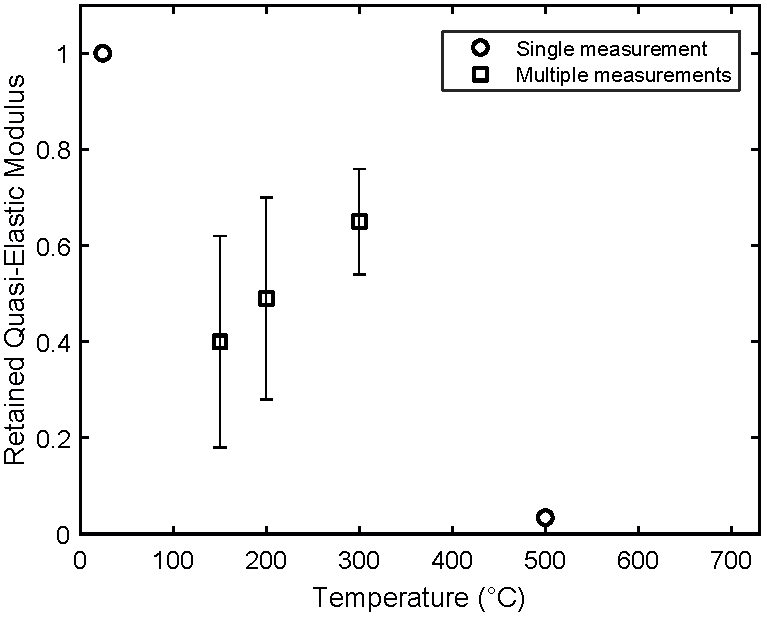
\includegraphics[width=0.90\linewidth]
		{Tex-Figures/Fig17b-qElast-Al.pdf}
		\caption{Aluminum foam}
		\label{fig:Quasi-elast-modulus_Al}
	\end{subfigure}
	\caption{ Quasi-elastic modulus.}
	\label{fig:Quasi-elast-modulus}
\end{figure}

\subsubsection{Quasi-Hardening Modulus}

As described above, following yield closed-cell foams exhibit significant plastic hardening, which differs from the elastic-perfectly material behavior where the hardening modulus is assumed to be close to zero. To determine the quasi-hardening modulus, Equation~\ref{Eq9} was fitted using global error minimization techniques to the entire experimental stress-strain curve for each specimen (shown in Figure~\ref{fig:Stress_strain_fit}).

The fitted parameters enable close approximation of the full stress-strain behavior of both HS steel and PM aluminum foams even throughout the densification phase. Table~\ref{Tab4}, located in the appendix, presents a summary of the fitted parameter values for each individual specimen. Figure~\ref{fig:Quasi-hardening-modulus} shows the resulting values of the quasi-hardening modulus as a function of temperature.

\begin{figure}
	\centering
	\begin{subfigure}{0.50\textwidth}
		\centering
		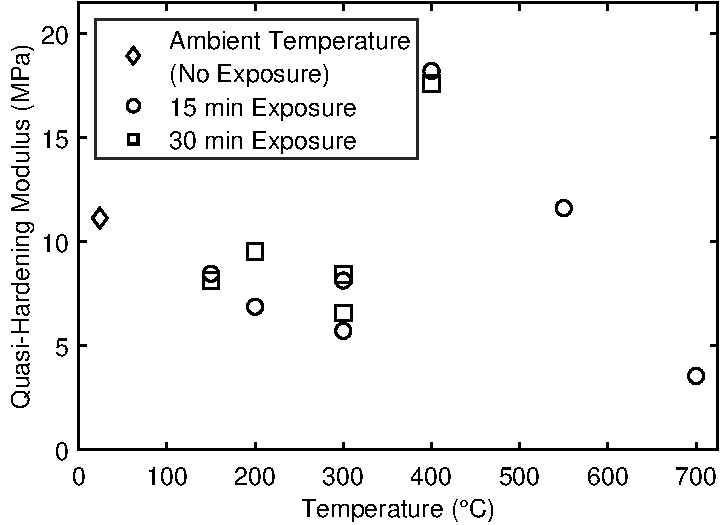
\includegraphics[width=0.90\linewidth]
		{Tex-Figures/Fig18a-quasi-Hardening-Fe.pdf}
		\caption{Steel foam}
		\label{fig:Quasi-hardening-modulus_Steel}
	\end{subfigure}% need comment here
	\begin{subfigure}{0.50\textwidth}
		\centering
		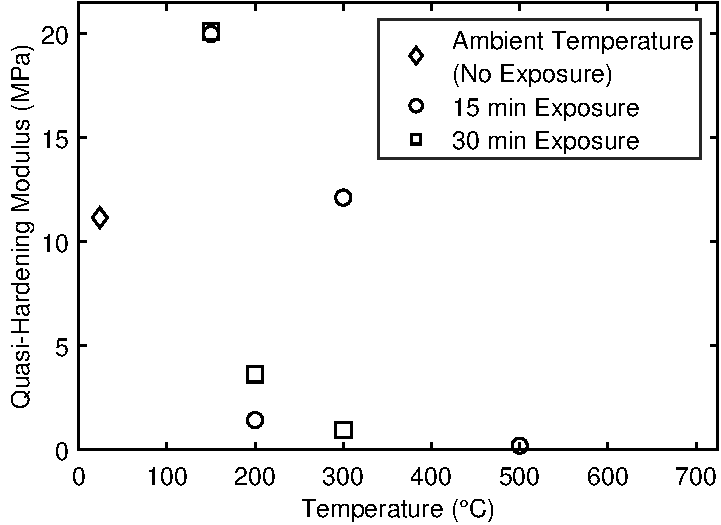
\includegraphics[width=0.90\linewidth]
		{Tex-Figures/Fig18b-quasi-Hardening-Al.pdf}
		\caption{Aluminum foam}
		\label{fig:Quasi-hardening-modulus_Al}
	\end{subfigure}
	\caption{ Quasi-hardening modulus did not degrade considerably for steel foam until 700~$^{\circ}\mathrm{C}$, while reduction of aluminum foam hardening modulus began manifesting itself at 300~$^{\circ}\mathrm{C}$.}
	\label{fig:Quasi-hardening-modulus}
\end{figure}


\subsubsection{Densification Strain}

The point of intersection of the two piecewise curves in Equation~\ref{Eq9} identically defines the inflection point between those segments. The strain location of this inflection point is designated in this study as the densification strain, or the strain at which the tangent slope of the stress-strain curve begins to increase relative to the hardening modulus thereby indicating densification of the metallic foam. Figure~\ref{fig:densification-modulus} does not show a clear influence of neither elevated temperatures nor exposure on the densification strain. Overall for both the HS steel and PM aluminum foams, the densification strain is scattered by approximately 0.08~mm/mm about a mean densification strain value of about 0.35~mm/mm.

\begin{figure}
	\centering
	\begin{subfigure}{0.50\textwidth}
		\centering
		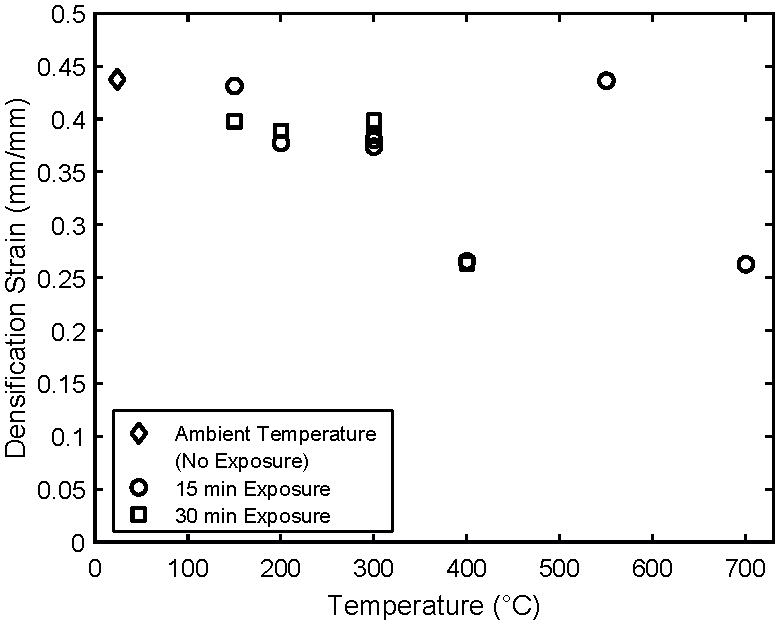
\includegraphics[width=0.90\linewidth]
		{Tex-Figures/Fig19a-densification-Fe.pdf}
		\caption{Steel foam}
		\label{fig:densification_Steel}
	\end{subfigure}% need comment here
	\begin{subfigure}{0.50\textwidth}
		\centering
		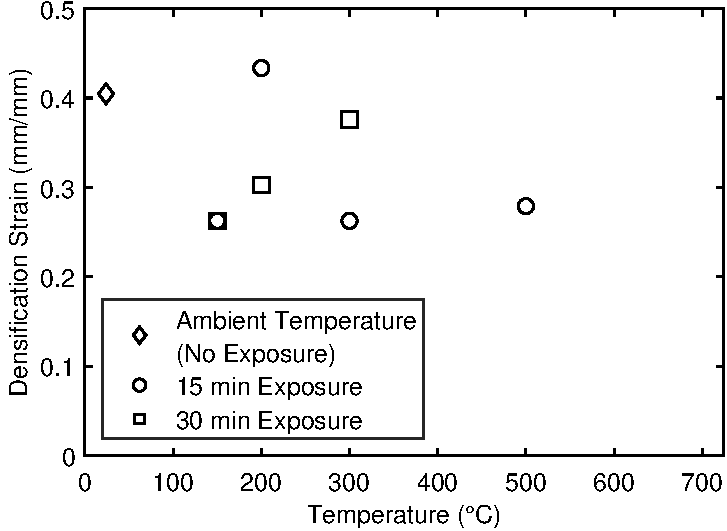
\includegraphics[width=0.90\linewidth]
		{Tex-Figures/Fig19b-densification-Al.pdf}
		\caption{Aluminum foam}
		\label{fig:densifiation_Al}
	\end{subfigure}
	\caption{ Quasi-hardening modulus did not degrade considerably for steel foam until 700~$^{\circ}\mathrm{C}$, while reduction of Al foam hardening modulus began manifesting itself at 300~$^{\circ}\mathrm{C}$.}
	\label{fig:densification-modulus}
\end{figure}


\subsubsection{Energy Absorption Efficiency}

While ISO Standard 13314:2011 does specify a methodology for calculating the energy absorption efficiency, this methodology first requires characterization of the densification strain which could only be reliably determined using the multi-parameter optimization approach described above. The energy absorption efficiency is calculated per ISO Standard 13314:2011 as the ratio of energy absorption capacity to the product of the maximum compressive stress (within the strain range spanning from 0.00~mm/mm to the densification strain), and the value of the densification strain (see Figure~\ref{EnAbsEffExpl}). The energy absorption capacity is shown as the hatched area in Figure~\ref{EnAbsEffExpl}, and the product of the maximum compressive stress within the strain range and the densification strain is the area bounded by the blue rectangle.

\begin{figure}[htbp]
	\begin{center}
		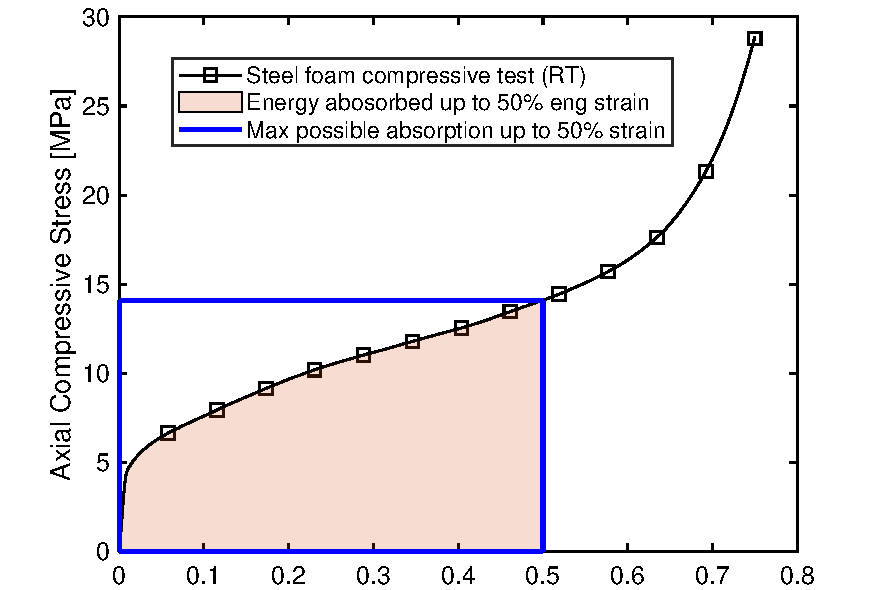
\includegraphics[width=0.60\linewidth]
		{Tex-Figures/Fig20-energyAbsorptionEfficiency.png}
		\vspace{-0.2cm}
		\caption{Schematic representation of methodology for calculating energy absorption efficiency.}
		\label{EnAbsEffExpl}
	\end{center}
\end{figure}

The energy absorption capacity is calculated either by integrating the stress-strain curve between strains of 0.00~mm/mm and 0.50~mm/mm, or by multiplying the plateau stress by 1.3. The integration-based approach was used in this study. As expected, trends in the behavior of the energy absorption capacity are similar to those of the plateau stress. Interesting, while the energy absorption capacity degrades more quickly with increasing temperature for the PM aluminum foam than for the HS steel foam, the energy absorption capacity of the two types of metallic foams is similar between temperatures of 150~$^{\circ}\mathrm{C}$ and 300~$^{\circ}\mathrm{C}$ (Figure \ref{fig:energyCapacity}). The exposure had relatively little influence on the energy absorption capacity for the HS steel foam; the energy absorption capacity for the two exposures did not differ by more than 4.0~\%. The energy absorption capacity of the PM aluminum foam was more scattered, but no systematic influence of exposure on the energy absorption capacity was observed.

\begin{figure}
	\centering
	\begin{subfigure}{0.50\textwidth}
		\centering
		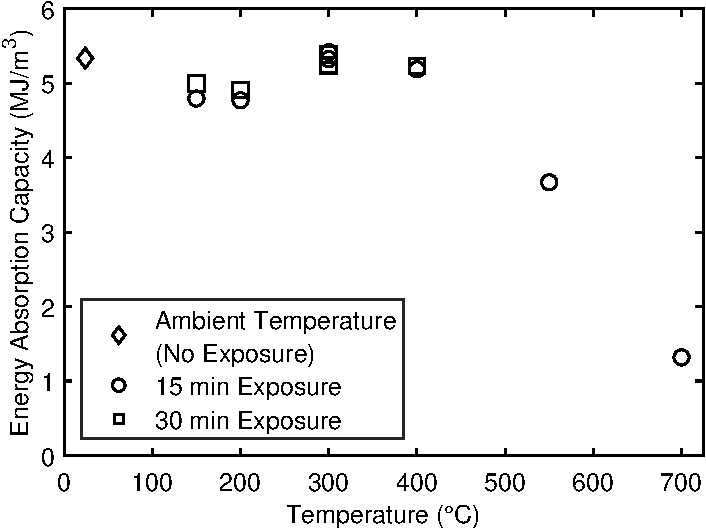
\includegraphics[width=0.90\linewidth]
		{Tex-Figures/Fig21a-EnergyCapacity-Fe.pdf}
		\caption{Steel foam}
		\label{fig:energyCapacity_Steel}
	\end{subfigure}% need comment here
	\begin{subfigure}{0.50\textwidth}
		\centering
		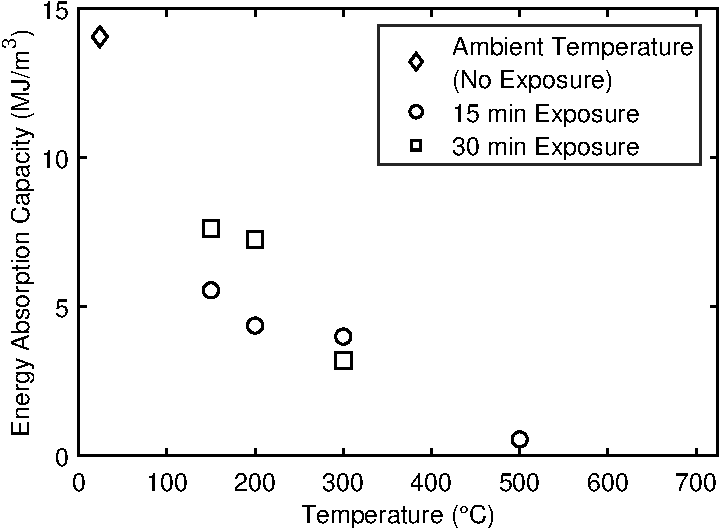
\includegraphics[width=0.90\linewidth]
		{Tex-Figures/Fig21b-EnergyCapacity-Al.pdf}
		\caption{Aluminum foam}
		\label{fig:energyCapacity_Al}
	\end{subfigure}
	\caption{ Energy absorption began degrading at 500~$^{\circ}\mathrm{C}$ for steel foam, while reduction for Al foam began manifesting itself at 150~$^{\circ}\mathrm{C}$.}
	\label{fig:energyCapacity}
\end{figure}

For the HS steel foam specimens, the energy absorption efficiency is nearly constant across all tested temperatures at a value of approximately 78~\%, and irrespective of the exposure (Figure~\ref{fig:energyEfficiency}). This trend implies that the shapes of the stress-strain curves are self-similar (at least up to the densification strain) and could be reproduced (in an approximate sense) by scaling the ambient temperature stress-strain response by a temperature dependent scalar reduction factor. Conversely, Aluminum foam exhibited hardening modulus approaching zero at higher temperatures and elastic perfectly plastic behavior with higher energy absorption efficiency.

\begin{figure}
	\centering
	\begin{subfigure}{0.50\textwidth}
		\centering
		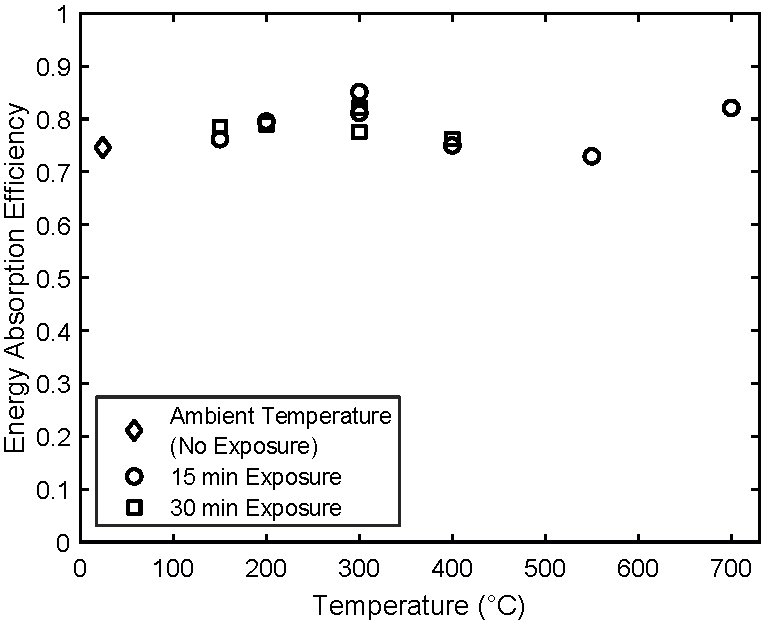
\includegraphics[width=0.90\linewidth]
		{Tex-Figures/Fig22a-energyEfficiency-Fe.pdf}
		\caption{Steel foam}
		\label{fig:energyEfficiency_Steel}
	\end{subfigure}% need comment here
	\begin{subfigure}{0.50\textwidth}
		\centering
		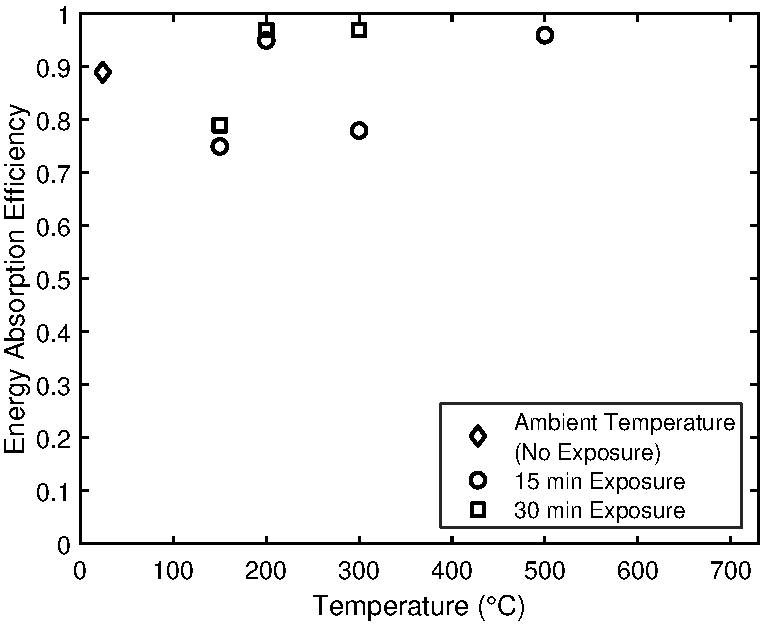
\includegraphics[width=0.90\linewidth]
		{Tex-Figures/Fig22b-energyEfficiency-Al.pdf}
		\caption{Aluminum foam}
		\label{fig:energyEfficiency_Al}
	\end{subfigure}
	\caption{ Energy absorption efficiency, calculated per ISO Standard 13314-2011 as the ratio of energy absorption capacity to the product of the maximum compressive stress (within the strain range spanning from 0.00~mm/mm to the densification strain). Energy absorption efficiency was constant for the steel foam, indicating that the thermal deterioration produced self-similar stress-strain curves. On the other hand, Aluminum foam showed increasing trend of the energy absorption efficiency, suggesting that while yield stress dropped sharply, the hardening modulus approached zero, and the material reached an almost elastic-perfectly plastic behavior, with corresponding high energy dissipation efficiency, but lower absolute value.}
	\label{fig:energyEfficiency}
\end{figure}

\section{Discussion}

The computational analyses revealed that the local capacity at the spherical shell length-scale, following initially elastic deformations, was controlled by the plastic buckling, mutual indentation, and bending of the spherical shells in contact. These contact regions are distributed randomly throughout the sample, resulting in localized plasticity. The deformation of the spheres is driven by bending of a spherical region, which increases radially as the material globally hardens. Random load paths complicate the development of closed-form multi-scale models linking local sphere geometry with the global macroscopic foam strength. Our computational observations compliment experimental studies by Gr\"{u}nder \cite{grunder_modeling_2001} and by Fallet et al. \cite{Fallet2008}, which also used CT-images to investigate internal foam deformations. Fallet proposed using the Weibull distribution to estimate the expected number of contact regions as a function of the overall global strain. Further work is needed to enable analytical predictions of the macroscopic foam properties from the geometry of the hollow spheres and their base metal properties through the use of statistics and elasto-plastic analytical modeling of the capacity of a spherical shell. Nevertheless, our simulations also indicated that the use of random variables for the sphere location and in the consideration of the packing pattern is necessary.

As expected from the fundamental buckling analysis of spherical shells, the thermal degradation of the metallic foams generally followed the temperature-induced reduction of yield stress of their respective base metals. Figure~\ref{fig:retention} compares the retention factors found in Eurocode (\cite{EC3-1-2}) for the solid, bulk steel and aluminum to the thermal degradation rate of the metal foams. The data for the HS steel foam followed the trends of the base metal with reasonable consistency. Note that Eurocode does not specify a specific time of exposure, but only states that the heating rate stay between 2~$^{\circ}\mathrm{C}$/min to 50~$^{\circ}\mathrm{C}$/min. Thus, it refers to the continuous exposure to the given temperatures. The testing conducted in this study did not show a significant influence of thermal exposure time (15~min or 30~min) on the thermal-mechanical properties of either the HS steel or PM aluminum foams.

According to EN 1999-1-2 \cite{EC9-1-2}, the mechanical properties of solid aluminum degrade at much lower temperatures than those of solid steel. Taherishargh et al. \cite{Taherishargh2018} previously reported that the reduction in material properties of foams follow the trend of the solid material. The yield stress of solid aluminum decreases by about 20~\% at 150~$^{\circ}\mathrm{C}$ and about 90~\% at 300~$^{\circ}\mathrm{C}$; the results for the PM aluminum foam followed a similar trend, but with even more significant reductions in strength (more than 50~\% at 150~$^{\circ}\mathrm{C}$ for some specimens, see Figure  \ref{fig:retention}). The mechanical performance of the PM aluminum foam was essentially negligible at temperatures exceeding 300~$^{\circ}\mathrm{C}$. These findings about aluminum foam behavior at elevated temperatures (compressive strength, energy absorption capacity and elastic modulus) are consistent with previous studies of aluminum foams in the literature (\cite{Aly2007}, \cite{Kovacicetal2016}, \cite{Liuetal2016}), and for the HS steel foams by \cite{BekozOktay2014}.

Although manufacturing of steel foam is more expensive than aluminum foam due to increased energy costs deriving from the higher melting point of steel, the retained strength and stiffness of HS steel foam at a given elevated temperatures is clearly larger than that of the PM aluminum foam. The Iron (Fe) based HS steel foam showed only minor degradation in mechanical performance at temperatures less than 400~$^{\circ}\mathrm{C}$, and retained 60~\% of its compressive strength at 550~$^{\circ}\mathrm{C}$. Such resilience might allow steel foam components to perform their intended functions even under elevated temperatures, by largely retaining the safety factors embedded in typical designs.

\begin{figure}
	\centering
	\begin{subfigure}{0.50\textwidth}
		\centering
		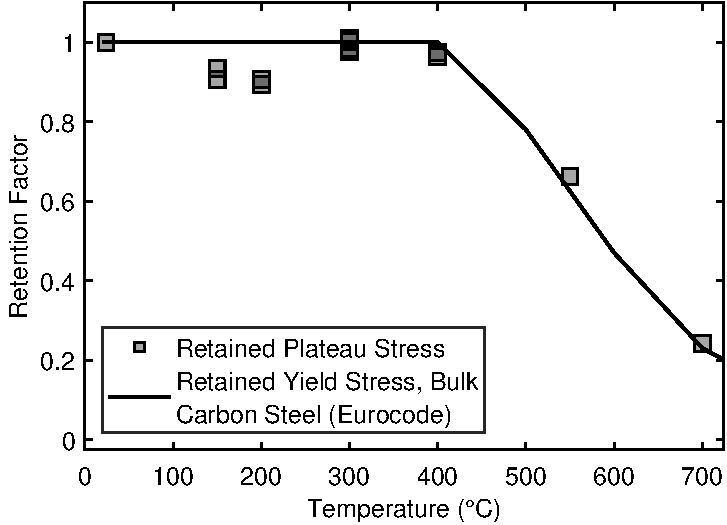
\includegraphics[width=0.90\linewidth]
		{Tex-Figures/Fig23a-retentionFactor-Fe.pdf}
		\caption{Steel foam}
		\label{fig:retention_Steel}
	\end{subfigure}% need comment here
	\begin{subfigure}{0.50\textwidth}
		\centering
		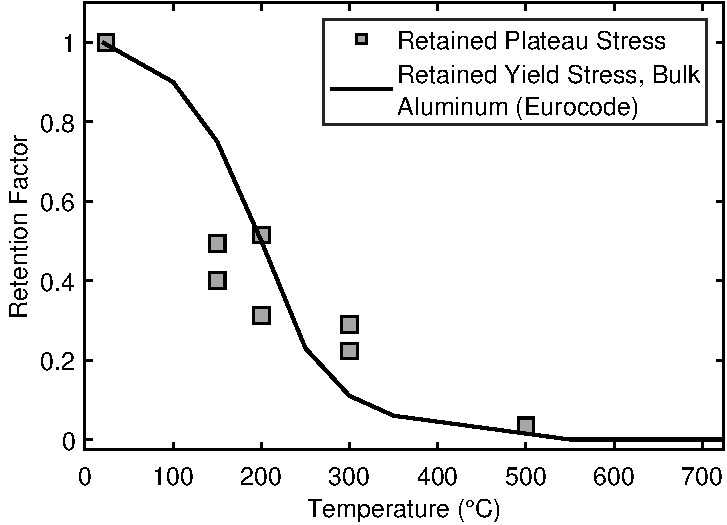
\includegraphics[width=0.90\linewidth]
		{Tex-Figures/Fig23b-retentionFactor-Al.pdf}
		\caption{Aluminum foam}
		\label{retention_Al}
	\end{subfigure}
	\caption{ Energy absorption efficiency, calculated per ISO Standard 13314-2011 as the ratio of energy absorption capacity to the product of the maximum compressive stress (within the strain range spanning from 0.00~mm/mm to the densification strain). Energy absorption was constant for the steel foam, indicating that the thermal deterioration produced self-similar stress-strain curves. On the other hand, Aluminum foam showed increasing trend, suggesting that wile yield stress dropped sharply, the hardening modulus approached zero, approaching almost elastic-perfectly plastic behavior, with corresponding high energy dissipation efficiency.}
	\label{fig:retention}
\end{figure}

The formation of a blue oxide surface skin during heating of HS steel foam specimens (see Figure \ref{fig:BlueOxide}) increased its stiffness within the temperature range of 200~$^{\circ}\mathrm{C}$ and 300~$^{\circ}\mathrm{C}$. These findings are consistent with Bekoz et al. \cite{BekozOktay2014}, who reported an increase in compressive yield strength and stiffness for PM steel foams for temperatures up to 400~$^{\circ}\mathrm{C}$, and a decrease above that temperature. Bekoz et al. \cite{BekozOktay2014} suggested an aging effect (dynamic age-hardening) as the reason for the increase in mechanical properties up to 400~$^{\circ}\mathrm{C}$ but did not detect any enhancement in the compressive strength over the temperature range.

Considering the large surface areas of metallic foams, surface-oxidizing chemical reactions could have a significant positive influence on the thermal-mechanical performance of steel foams. For example, pre-oxidization of FeCrAl enhances its mechanical properties at temperatures up to 400~$^{\circ}\mathrm{C}$. The potential for such reactions to reliably increase thermo-mechanical performance should be also investigated for other base metals and alloys because these reactions could allow metallic cellular structures to outperform their constituent base metals.

\section{Summary and Conclusions}

The compressive behavior of hollow sphere (HS) steel foam and powder metallurgy (PM) aluminum foams were studied at elevated temperatures to characterize their thermo-mechanical properties. The experimental results showed that the HS steel foam retained more than 89~\% of its compressive strength, when measured by the plateau stress, up to 400~$^{\circ}\mathrm{C}$, and 69~\% of its strength and energy absorption capacity at 550~$^{\circ}\mathrm{C}$. At 700~$^{\circ}\mathrm{C}$, much of the structural integrity of the HS steel foam was largely diminished, retaining only 24~\% of its compressive strength and energy absorption capacity. Contrarily, the PM aluminum foam retained only about 45 \% of its strength and energy absorption capacity at 150~$^{\circ}\mathrm{C}$, and had virtually no strength (only 3.5~\%) remaining at 500~$^{\circ}\mathrm{C}$.

High-resolution computational models showed that, under increased deformation, plasticity spreads toward the equators of individual hollow spheres, gradually increasing the diameter of their plastic hinge hoops until buckling of the sphere-walls occurred. This observation was further supported by analytical consideration of buckling of a spherical shell. Thus, the local plasticity and plastic stress are critical for the thermal deterioration of metallic foams' mechanical capacities because they control local plastic buckling. As anticipated from the simulations, the retained plateau stress for both the HS steel and PM aluminum foams generally followed the elevated-temperature degradation of the yield stress of their respective base metals (available from Eurocode EN 1993-1-2:2005 and EN 1999-1-2:2007). However, based on the general buckling stability considerations, it might be possible to manufacture ultra-thin-walled foams, which should exhibit highly elastic, reversible deformations. Their thermal behavior would be expected to follow thermal deterioration of modulus of elasticity of the base material. This observation is consistent with previously reported hyper elastic behavior of ultra-thin-walled hollow lattice structures \cite{Sch2011}.

The experiments also revealed an interesting chemical phenomenon. A blue oxide film formed on the surface of the steel foam. This film was likely responsible for the moderate increases of quasi-elastic gradient between temperatures of 200~$^{\circ}\mathrm{C}$, 300~$^{\circ}\mathrm{C}$, higher stress-strain curves in the range of 300~$^{\circ}\mathrm{C}$ to 400~$^{\circ}\mathrm{C}$ then 100~$^{\circ}\mathrm{C}$ as well as discrepancy between the simulated and experimental stress strain curves of HS steel foam at higher temperatures.  Chemical reactions that occur at elevated temperatures will be considered in future studies because they might allow metallic foams to exceed thermo-mechanical performance of their base metals by taking advantage of the large surface area to volume ratio in cellular structures.

The high thermal resilience of steel foams suggests that their potential range of application might extend to temperatures traditionally precluded for polymeric or even aluminum foams. The energy absorption capacity of the HS steel foam was nearly constant at the temperatures below 400~$^{\circ}\mathrm{C}$, and significant residual energy absorption capacity (about 69~\%) remained at 550~$^{\circ}\mathrm{C}$. In addition, the energy absorption efficiency was essentially constant at about 80~\% and did not diminish at elevated temperatures. Thus, steel foams may be suitable for dissipation of impacts, crashes or other extreme loads at elevated temperatures. The crashworthiness could be combined with heat exchange functions in open cell foams. This research is a part of broader effort to develop understanding of cellular metallic materials with relevance to aerospace, automotive, energy and infrastructure applications.

\begin{table}[htbp]
	\begin{tabular}{ll}
		\textbf{List of Acronyms} \\
		HS    & Hollow Sphere \\
		PM    & Powder Metallurgy \\
		ISO   & International Organization for Standardization \\
		IFAM  & Fraunhofer Institute for Manufacturing Technology and Advanced Materials \\
		MTS   & Material Testing System \\
		UTM   & Universal Testing Machine \\
		RCP   & Random close-packed \\
		RT    & Room Temperature \\
		SF    & Steel Foam \\
		AF    & Aluminum Foam \\
		METFOAM & International Conference on Porous Metals and Metallic Foams \\
		EPSRC & Engineering and Physical Science Council
	\end{tabular}%
\end{table}%

\FloatBarrier

\renewcommand{\nomname}{List of Symbols}

% Equation 1
%\nomenclature{$r_{p r o j}^{i}$}{Projected Radius used for measuring the size of the spherical pore}
%\nomenclature{$r_{t r u e}$}{True Radius of the spherical pore size}
%\nomenclature{$h_{proj}^{i}$}{Height of the random cut plane used for measurement of the spherical pore size}

% Equation 2
%\nomenclature{$\alpha$}{Correction factor used for the  measurement of the spherical pore size}

% Equations 3 and 4
%\nomenclature{R}{Sphere radius}
%\nomenclature{t}{Sphere Thickness}
%\nomenclature{$\sigma_{shell}$}{Buckling Stress of Spherical Shell}
%\nomenclature{$q_{c}$}{Pressure applied to a sphere}
%\nomenclature{$d_{c}$}{Diameter of the contact area between the spheres}

% Equation 5
%\nomenclature{$\sigma_{c r}$}{Critical limit of membrane stress}
%\nomenclature{E}{Young Modulus}
%\nomenclature{$\mathcal{V}$}{Poisson ratio}

% Equation 6
%\nomenclature{$\sigma_{failure}$}{Failure Stress}
%\nomenclature{$\sigma_{y}$}{Yield stress}

% Equation 7
%\nomenclature{$\lambda$}{Slenderness}


% Figure 7
%\nomenclature{$E_{i}$}{Initial elastic modulus}
%\nomenclature{$E_{p}$}{Plastic hardening modulus}
%\nomenclature{$n_{y}$}{Shape parameter that controls the sharpness of the transition from the elastic stiffness to the plastic stiffness}
%\nomenclature{$f_{y}$}{Yield stress calculated using the 0.2% offset method}
%\nomenclature{$\sigma_{p l}$}{Plateau Stress}


% Figures 12a and 12b
%\nomenclature{$\sigma_{y}^{shell}$}{Yield stress of the spherical shell}
%\nomenclature{$\sigma_{cr}^{shell}$}{Critical stress of the spherical shell}


% Equations 8, 9 and 10
%\nomenclature{q}{Applied pressure}
%\nomenclature{$\varphi$}{Polar coordinate, where 0 corresponds to the equator and pi/2 to the apex of the sphere}
%\nomenclature{$\omega_{a p e x}$}{Deformation of the sphere apex under uniform pressure}

% Equations 11 and 12
%\nomenclature{$\sigma_{d}$}{Densification Stress that define the transition to stiffening behavior}
%\nomenclature{$E_{i}(\mathrm{T})$}{Initial elastic modulus at high temperature}
%\nomenclature{$E_{p}(\mathrm{T})$}{Plastic hardening modulus at high temperature}
%\nomenclature{$\varepsilon$}{Compressive strain}
%\nomenclature{$\varepsilon_{d}$}{Densification Strain that define the transition to stiffening behavior}
%\nomenclature{$E_{b}(\mathrm{T})$}{???}
%\nomenclature{$E_{d}(\mathrm{T})$}{Densification stiffness}
%\nomenclature{$\varepsilon_{d}(\mathrm{T})$}{Densification stiffness}
%\nomenclature{$\sigma_{p}(\mathrm{T})$}{Projection of densification stress at zero strain}
%\nomenclature{$n_{b}(T)$}{Shape parameter that controls the sharpness of the transition from the plastic stiffness  to the densification stiffness  at high temperature, Figure 7}
%\nomenclature{$n_{y}(T)$}{Shape parameter that controls the sharpness of the transition from the elastic stiffness  to the plastic stiffness  at high temperature}
%\nomenclature{T}{Temperature}

% Page 26
%\nomenclature{$\varepsilon_{y}$}{Yield strain calculated using the 0.2\% offset method}

\printnomenclature[1.5cm]

\section*{Acknowledgements}

The authors would like to express heartfelt gratitude to our academic colleagues for their feedback and fruitful discussions. We are grateful to Fraunhofer IWU in Chemnitz and Fraunhofer IFAM in Dresden for the ongoing collaboration, and for their help with supplying the metallic foam rectangular prisms for mechanical testing. We would like to thank Dr Rene Vogel, Dr Thomas Hipke, Dr Olaf Andersen, Dr Peter Quadbeck and Dr Christian Hannemann.

We also would like to express our gratitude to technicians who assisted us during the mechanical tests, namley Mr Peter Heynes and David Jesson. We are also indebted to LS-DYNA support and developers for their assistance with the implicit, large deforamtion and large-strain micro-model.

This study was funded by the Research Framework of the European Commission under METFOAM Career Integration Grant 631827 with support from program manager Dr. Ing. Antonio Cipollaro. The work was also supported by the impact acceleration grant no EP/P511456/1, provided by the Engineering and Physical Science Council (EPSRC) in the UK. Support of Dr. Sue Angulatta, a local program manager, is genuinely appreciated. Any opinions, findings, and conclusions expressed in this article are those of the author(s) and do not necessarily reflect the views of EPSRC or the European Commission.


\section*{Data availability}

The data is available upon request from the corresponding author.

\bibliography{FirepaperBibfile}

\section*{Appendix}

\subsection*{Fitted Richard Equation Parameters}

The Richard Equation parameter values fitted only to elastic phase of each specimen's stress-strain response are presented in Table \ref{Tab3}, and the Richard Equation parameter values fitted to each specimen's full stress-strain curve are presented in Table \ref{Tab4}.

\begin{landscape}


% Table generated by Excel2LaTeX from sheet 'Sheet2'
\begin{table}[htbp]
	\centering
	\caption{Richard Equation Parameters fitted only to Elastic Phase of Specimen Stress-Strain Curve.}
	\begin{tabular}{cccccccccc}
		\toprule
		Spec. &   $E_i(T)$    &   $E_p(T)$    &  $\sigma_y(T)$     &   $n_y(T)$     &    $E_b(T)$   &    $E_d(T)$   &   $\sigma_p(T)$    &   $n_d(T)$    &  $(\varepsilon_d,\sigma_d)$\\
		\midrule
		SF\_T24C & 611   & 76.9  & 4.4   & 10.01 & -     & -     & -     & -     & - \\
		SF\_T150C\_15 & 979   & 166.8 & 2.8   & 5.59  & -     & -     & -     & -     & - \\
		SF\_T150C\_30 & 916   & 156.5 & 3.4   & 7.71  & -     & -     & -     & -     & - \\
		SF\_T200C\_15 & 1487  & 3.7   & 4     & 2.39  & -     & -     & -     & -     & - \\
		SF\_T200C\_30 & 1351  & 84.8  & 4.5   & 4.98  & -     & -     & -     & -     & - \\
		SF\_T300C\_15(1) & 1770  & 381   & 2     & 2.79  & -     & -     & -     & -     & - \\
		SF\_T300C\_15(2) & 745   & 246.1 & 2.8   & 5.9   & -     & -     & -     & -     & - \\
		SF\_T300C\_30(1) & 1084  & 238   & 2.5   & 3     & -     & -     & -     & -     & - \\
		SF\_T300C\_30(2) & 730   & 183.1 & 3.3   & 6.19  & -     & -     & -     & -     & - \\
		SF\_T400C\_15 & 613   & 157.4 & 3     & 7.6   & -     & -     & -     & -     & - \\
		SF\_T400C\_30 & 670   & 58.9  & 4.4   & 3.43  & -     & -     & -     & -     & - \\
		SF\_T550C\_15 & 1017  & 78.8  & 3.4   & 2.6   & -     & -     & -     & -     & - \\
		SF\_T700C\_15 & 734   & 35.9  & 1.3   & 2.3   & -     & -     & -     & -     & - \\
		AF\_24C & 2514  & 327.2 & 15.2  & 2.62  & -     & -     & -     & -     & - \\
		AF\_T150C\_15 & 625   & 205.9 & 3.6   & 9.12  & -     & -     & -     & -     & - \\
		AF\_T150C\_30 & 1397  & 204.1 & 6.9   & 3.88  & -     & -     & -     & -     & - \\
		AF\_T200C\_15 & 840   & 166.9 & 5.5   & 6.21  & -     & -     & -     & -     & - \\
		AF\_T200C\_30 & 1602  & 347.4 & 7.7   & 4.81  & -     & -     & -     & -     & - \\
		AF\_T300C\_15 & 1437  & 85.6  & 5.1   & 3.5   & -     & -     & -     & -     & - \\
		AF\_T300C\_30 & 1820  & 48    & 6.2   & 2.2   & -     & -     & -     & -     & - \\
		AF\_T500C\_15 & 86    & 2.2   & 0.8   & 9.54  & -     & -     & -     & -     & - \\
		\bottomrule
	\end{tabular}%
	\label{Tab3}%
\end{table}%


% Table generated by Excel2LaTeX from sheet 'Sheet2'
\begin{table}[htbp]
	\centering
	\caption{Richard Equation Parameters fitted to Specimen Full Stress-Strain Curve.}
	\begin{tabular}{cccccccccc}
		\toprule
		Spec. &  $E_i(T)$     &    $E_p(T)$   &   $\sigma_y(T)$    &   $n_y(T)$    &     $E_b(T)$   &    $E_d(T)$   &   $\sigma_p(T)$    &   $n_d(T)$    &  $(\varepsilon_d,\sigma_d)$\\
		\midrule
		SF\_T24C & 15697 & 11.1  & 11.8  & 0.35  & 0.44  & 18.7  & 84.6  & 13.1  & 9.36 \\
		SF\_T150C\_15 & 12219 & 8.5   & 11.5  & 0.35  & 0.43  & 13.7  & 54    & 9.3   & 3.98 \\
		SF\_T150C\_30 & 22337 & 8.1   & 11.2  & 0.35  & 0.4   & 13.6  & 50.9  & 8.2   & 8.32 \\
		SF\_T200C\_15 & 15550 & 6.9   & 11.8  & 0.34  & 0.38  & 12.3  & 44.1  & 6.8   & 9.14 \\
		SF\_T200C\_30 & 3841  & 9.5   & 8.4   & 0.6   & 0.39  & 16.5  & 64.8  & 10.8  & 15.15 \\
		SF\_T300C\_15(1) & 3322  & 8.1   & 10.2  & 0.6   & 0.38  & 15.9  & 43.9  & 11.7  & 100.28 \\
		SF\_T300C\_15(2) & 1146  & 5.7   & 9.8   & 0.99  & 0.37  & 15.9  & 66.8  & 12.1  & 107.82 \\
		SF\_T300C\_30(1) & 14081 & 8.4   & 13.3  & 0.35  & 0.4   & 17.1  & 63.3  & 9.6   & 20.33 \\
		SF\_T300C\_30(2) & 3798  & 6.6   & 10.5  & 0.56  & 0.38  & 16.7  & 66.4  & 10.9  & 38.01 \\
		SF\_T400C\_15 & 2554  & 18.2  & 6.3   & 0.84  & 0.27  & 15.1  & 51.8  & 12.3  & 6.61 \\
		SF\_T400C\_30 & 1252  & 17.6  & 6.5   & 1.17  & 0.26  & 14    & 45.5  & 9.7   & 12.37 \\
		SF\_T550C\_15 & 1191  & 11.6  & 4.4   & 1.83  & 0.44  & 25    & 101.9 & 8.5   & 5.5 \\
		SF\_T700C\_15 & 649   & 3.5   & 1.8   & 1.63  & 0.26  & 2.9   & 12.3  & 3.1   & 8.03 \\
		AF\_24C & 2565  & 11.2  & 26.1  & 1.44  & 0.4   & 37.2  & 199.6 & 29.6  & 5.77 \\
		AF\_T150C\_15 & 1195  & 20    & 6.7   & 1.58  & 0.26  & 9.2   & 62.7  & 13.6  & 3.81 \\
		AF\_T150C\_30 & 1393  & 20.1  & 9.2   & 3.65  & 0.26  & 39.8  & 75.8  & 10    & 39.83 \\
		AF\_T200C\_15 & 961   & 1.4   & 8.5   & 3.39  & 0.43  & 2.9   & 43.8  & 11.3  & 0.79 \\
		AF\_T200C\_30 & 1694  & 3.6   & 13.7  & 2.4   & 0.3   & 3.6   & 67.6  & 15.9  & 20.5 \\
		AF\_T300C\_15 & 1666  & 12.1  & 5.3   & 3.93  & 0.26  & 5.5   & 45.9  & 10.6  & 4.18 \\
		AF\_T300C\_30 & 2165  & 0.9   & 6     & 2.68  & 0.38  & 3.7   & 59.4  & 11.8  & 1.86 \\
		AF\_T500C\_15 & 3774  & 0.2   & 1     & 0.78  & 0.28  & 0.7   & 6.8   & 2.2   & 1.3 \\
		\bottomrule
	\end{tabular}%
	\label{Tab4}%
\end{table}%

\end{landscape}

\end{document}
